\documentclass[onecolumn,12pt]{article}

\usepackage[left=1in,right=1in,top=1in,bottom=1in]{geometry}

\usepackage{latex8}
\usepackage{epsfig}
\usepackage{url}
\usepackage{times}
%\usepackage[rflt]{floatflt}
\usepackage{fancyhdr}
\usepackage{subfigure}
\usepackage{cite}
\usepackage{xspace}
\usepackage{color}
\usepackage{wrapfig}
\usepackage{multirow}
\usepackage{amsmath}
\usepackage{colortbl}
\usepackage{cancel}
\usepackage{umoline}
\usepackage{setspace}
\usepackage{titling}
\usepackage[table]{xcolor}

\setlength{\intextsep}{3pt}
\setlength{\columnsep}{3pt}


\begin{document}

\pagenumbering{gobble}
    
\title{Authentic Contextualization in \\Computer Science Education with Big Data:\\ Pedagogy, Motivation, and Technology} 

\author{Austin Cory Bart}
% Revisit title
\maketitle     
    
\newpage   
\section{Summary}

This preliminary proposal explores introductory computing contexts, and suggests a research plan to evaluate its motivational impact on students.
In particular, it focuses on the use of Datasets and Data Science as an introductory context as a holistically motivating context that can authentically appeal to a wide ranger of learners.
I propose to design pedagogical materials and technologies to integrate datasets into courses.
This research will move past traditional research on using data science for education, which currently is limited to brief case studies with little to no evaluation.
Instead, it will focus on serious evaluation and the principled, detailed analysis of how the affordances, issues, and value of this context.
It will be comparative to existing research on other introductory contexts such as Media Computation or Game/Animation Design.
Additionally, it will have a strong focus on new technological solutions to support the learning process, leveraging computational techniques in software engineering and data analysis.
It will also contribute to the ongoing research onto the effect of motivation on academic success, in particular the novel application of the MUSIC Model.


    
\newpage
\pagenumbering{arabic}
\setcounter{page}{1}
        
    \section{Problem Statement}

A report by MGI and McKinsey's Business Technology Offices declares that ``... by 2018, the United States alone could face a shortage of 140,000 to 190,000 people with deep analytical skills as well as 1.5 million managers and analysts with the know-how to use the analysis of Big Data to make effective decisions''~\cite{McKinsey} .
This gap, and the expanding recognition of ``Computational Thinking'' as a 21st century skill, increasingly requires that computation be positioned in a university's general education curriculum~\cite{wing2006}.
For instance, Virginia Tech is now formalizing this requirement through a new course (``Introduction to Computational Thinking'') that all university students will eventually be required to take~\cite{vt-vision}.
Such a course poses serious pedagogical and motivational challenges: how do we introduce Computational Thinking to students with no prior computing experience and convince them that the field can tangibly benefit their respective disciplines?



We need more students in Computer Science and with Computational skills
Describe introductory programming
CS-1,2,3: Quick one-sentence descriptions
As students progress to CS-3, motivation becomes less critical compared to self-regulation
CS-0:  "Computational Thinking"
Limited time to teach relevant concepts
Desire to engage them
In order to bring in these students, we must approach this from both the cognitive and motivational sides
Want to keep students highly motivated
Decontextualized assignments
But we also have a new set of skills to teach students
Data science
Big Data
What can technology and pedagogy do to solve this problem
In this preliminary proposal, we describe work previously done and future work


Computer Science and Computational Thinking
New audiences



Introductory programming
	CS-1,2,3
	Computational Thinking
		Wing definition
Contextualization
	Abstract
		Straw-man example of boring lists
	Constructivism
	Socio-constructivism
	Situated Learning
	Authentication
		Preauthentication
		Over-authentication (?) - I like dinosaurs, but you suck at teaching dinosaurs
Scaffolding
	Fading
Media Computation
	Pre-authentication - students won't find it realistic to their experiences
	Under-authentication - not realistic enough for the students tastes
	Over-authentication - overly engaging and distracting (Seductive Details)
	
	http://dl.acm.org/citation.cfm?id=2493397
Proposed Theory
	Retention hypothesis
	Gender Hypothesis
	Learning Hypothesis
		Gains vs. Absolute
	More-Computing Hypothesis
		Code Aacdemy, Let's Code Blacksburg
	
Prior Work
	Real-time Web
Proposed Architecture
	+Big-Data
	+Sources
	Python + Blockly
Proposed curriculum
	Usable as components or a whole
	Good for students motivated by usefulness
Work Plan


Big Data is much in the news these days, from reports of massive data
dredging by the NSA to tens of millions of credit cards stolen by
hackers from commercial databases.
Big Data has become crucial to scientific advances from understanding the
genome to predicting climate change.
It would do well for anyone these days to appreciate the capabilities
and the limits of Big Data processing.
Certainly a study of Big Data concepts aligns well with current
efforts to acquaint a broad range of students to Computational
Thinking, and it certainly would be of broad interest to most of these
students.

Leveraging the promise of Big Data offers unprecedented opportunities
for improved economic growth and enhanced innovation.
Unfortunately, computer scientists in the workforce are woefully
unequipped for this shifting paradigm.
Indeed, a report by MGI and McKinsey's Business Technology Offices
declares that ``by 2018, the United States alone could face a
shortage of 140,000 to 190,000 people with deep analytical skills as
well as 1.5 million managers and analysts with the know-how to use the
analysis of Big Data to make effective decisions.''\cite{McKinsey}
In order to close this gap, we need to do more than just improve the
education of existing students; we must draw from under-represented
and non-traditional sectors.
In particular, we need to start reaching out to non-majors through the banner of Computational Thinking.

There are two main obstacles to effectively educating students on Big
Data.
First, its representation, manipulation, and expression is
challenging, with modern curriculums and programming tools being
inadequate.
In fact, the definition of Big Data is quantities of information that
cannot be handled with traditional methods\cite{McKinsey}.
Second, postponing these topics until late in the curriculum, as is
commonly done\cite{CS2013}, fails to prepare students to solve problems in this
domain; the Computer Science Curricula 2013 recommends 10 core hours
minimum, requiring more distribution of the material over the life of
an undergraduate program.
Moreover, learning how to manage this complexity is central to
interdisciplinary work in everything from agriculture to medicine to
law, and everything in between\cite{theory-end}.
We cannot expect non-majors to progress too far through our own
subject, so therefore work must be done to cover this material in
introductory courses, as early and often as possible.

Despite the difficulties, there are serious benefits to introducing Big Data problems earlier into the curriculum.
By opening an entire new class of problems, assignments can be more varied.
By exposing students to Big Data topics earlier, their foundational understanding will be stronger and they will develop a stronger interest in this important subject.
And finally, we can introduce non-majors to useful skills that they can immediately apply to their own subjects, fostering interdisciplinary work.
But how do we make this complicated and difficult topic accessible?
    \section{Educational Theories}

There are many theories of how people learn, how to teach, and how to engage with students. 
In this section of the proposal, we review dominant theories that guide the research.
First, we will discuss how people learn, and the dominant theories that guide researchers.
Then, we will discuss Instructional Design, which is concerned with how to support the learning process.
Finally, we will look at motivation and engagement, the reason people choose to direct their energy towards goals.

\subsection{Theories of Learning}


There are many, many theories of learning, far more than can be accurately captured here.
However, there are a few major paradigms worth discussing briefly: Cognitivism, Constructivisim, and Behavioralism.
Cognitivism emerged as a response to classical theories on Behaviorist learning -- the latter posits learning as a ``black box'' process, and the former encourages researchers to ``pry open the box'' \cite{learningtheories}.
This in turn led to the development of Constructivism, which describes learning as an active process of linking knowledge based on prior, subjective experiences.
These theories are not replacements for each, but lenses for analyzing different learning experiences. Cognitivism and Constructivism in particular are usually more useful for studying higher learning.

\subsubsection{Situated Learning Theory}

Situated Learning Theory, originally proposed by Lave and Wenger, argues that learning normally occurs as a function of the activity, context, and culture in which it is situated\cite{lave-situated}.
Therefore, tasks in the learning environment should parallel real-world tasks, in order to maximize the \textit{authenticity}.
Contextualization is key in these settings, as opposed to decontextualized (or ``inert'') settings.
The key difference is that learning is driven by the problem being solved, rather than the tools available – therefore, the problem being solved should lead directly to the tool being taught.

A critical element of these situated environments is the need for social interaction and collaboration, as learners become involved in and acculturated by ``Communities of Practice'' \cite{brown1989situated}.
Members of a CoP share purposes, tools, processes, and a general direction -- they should have a commonly recognized domain. 
This interaction occurs not only between individuals and the experts of the community (commonly represented by teachers) in an apprenticeship model, but also occurs between different learners as they adapt at uneven paces.
This communication between peers leads to growth among both individuals, especially when access to authentic experts is limited.
As the learner develops into an expert, they shift from the outside of the community's circle to the center, becoming more and more engaged -- this is the process of ``Legitimate Peripheral Participation''.

Authenticity is another crucial, recurring theme within Situated Learning Theory.
All instruction and assessment must be aligned with reality such that success in the former leads to success in the latter.
However, there is a subtle nuance here -- authenticity is a perceived trait, not an objective one.
Students derive value from their learning only if they \textit{perceive} authenticity, regardless of whether the instructor has successfully authenticated the experience.

Situated Learning Theory has been applied to the domain of Computer Science before, with mixed results. A seminal paper by Ben-Ari \cite{ben2004situated} explores its application and limitations.
This paper is somewhat hasty in its application of SL Theory by taking a macro-level view -- they narrowly look to Open-Source and Industry Software Development communities as the only potential CoPs and interpret SL Theory as strictly requiring constant legitimacy, largely ignoring the possibility for gradual development of authenticity within individual courses and modules throughout a curriculum:

\begin{quote}
What I am claiming is that situated learning as presented in their work cannot be accepted at face value, because it simply ignores the enormous gap between the world of education and the world of high-tech CoPs, which demand extensive knowledge of both CS subjects and applications areas.
This gap can only be bridged by classical decontextualized teaching in high schools, colleges and universities.
\end{quote}

However, other researchers have found it a useful lens for analyzing curricula.
For instance, Guzdial and Tew \cite{guzdial2006imagineering} used the theory to innovatively explore and deal with the problem of inauthenticity within their Media Computation project.
SL Theory clearly has value, but only as a function of the way that it is applied.
In this preliminary proposal, I will take advantage of SL Theory as a generalized tool for exploring the topic of authenticity throughout introductory Computer Science.

The original work in Situated Learning Theory was categorically not about pedagogy or instructional design- it described how people learn and the importance of context and collaboration, but it did not recommend a particular style of classroom.

\subsection{Theories of Instructional Design}

Instructional Design is the systematic design of effective Learning Experiences. One of the most influential\cite{anglin1992reference} instructional theories is Gang\'{e}'s Theory of Instruction, a complex Cognitivist model that categorizes different types of learning outcomes (e.g., ``Verbal Information'' such as reciting the definition of a term, ``Attitudinal'' such as choosing to not smoke) and breaks down the process of learning into nine coherent steps. Gang\'{e} stresses that different learning outcomes require very different instructional implementations of the general instructional model. This instructional theory informs the design of complete Instructional Design models such as the Dick and Carey model \cite{carey2001systematic}. Although different ID models suggest different approaches to creating instructional materials, those materials are all typically patterned after Gang\'{e}'s instructional events.

\subsubsection{Gagn\'{e}'s Instructional Events}

\begin{figure}
\begin{description}
	\item[(1) Gain Attention:] Stimulate the learner and motivate them to engage with the material.
	\item[(2) Describe Objectives:] Inform the learner will be able to do because of the instruction.
	\item[(3) Stimulating Recall of Prior Knowledge:] Remind students of their prior knowledge.
	\item[(4) Present the Material:] Using text, graphics, etc., give the instructional materials.
	\item[(5) Provide Guidance:] Give instructions on how to use the instructional materials.
	\item[(6) Elicit Performance:] Have the learners actively apply the new knowledge.
	\item[(7) Provide Feedback:] Show the learner what they did well and poorly on.
	\item[(8) Assess Performance Test:] Evaluate the learner on their performance
	\item[(9) Enhance Retention and Transfer:] Generalize the instruction by showing similar applications.
\end{description}
\caption{Gang\'{e}'s Nine Events of Instruction}
\label{gange-events}
\end{figure}

Gang\'{e}'s nine events are summarized in Figure \ref{gange-events}, taken indirectly from\cite{gagne1985conditions}. This model is described as an ordered, one-way sequence; however, in practice, some steps might be repeated and cycled between. For instance, very negative feedback might prompt the learner to return from step 7 to step 6. Modifications of the model have also been discussed in the literature. For example, to adapt for more Constructivist tastes, one could swap steps 4 and 6, so that students have the opportunity to engage with the materials before receiving instruction.

Instructional Designers often identify three key interactions in a learning experience. In the simplest case, an instructor presents some new material, a learner participates in questions related to it, and the instructor assesses their performance as being excellent. Although it might appear that Gagn\'{e}'s model maps presentation to steps 1--5, participation to step 6, and assesssment to 7--9, this is an over-simplification of a much richer set of interactions. For instance, step 1 (Gain Attention) often involves a dialogue or other participation from the students, and step 7 often requires re-presentation of existing material or presentation of new material. In practice, every learning experience will end up being a unique combination of these interactions.

Instructors and learners are involved in all of these interactions in different capacities and degrees. Presentation is primarily a flow of information from the Instructor to the learner. Participation is primarily an externalization of knowledge by the learner for the Instructor. Assessment is a mediation between the Instructor and the learner to align the externalization.

Instructional Design Models such as Dick \& Carey usually delay the design of instructional materials till the end of the entire process, focusing initially on analysis of the learners, the performance context, the instructional goal, and a host of other critical factors. At that point, a content delivery system is chosen based on its educational affordances and suitability for the learning experience being developed. This delay reflects the typical role of an Instructional Designer as a \textit{consumer} of instructional technology -- they survey the available techniques and technology (e.g., traditional lecture, essay writing, websites), and choose the one that fits their need. In the remainder of this paper, we use instead take the Software Designer role of \textit{producer} of instructional technology in order to analyze some of the decisions that go into the design of these environments, from the retrospective of an Instructional Designer.

\subsubsection{Situated Learning Environment Design}

Situated Learning Theory is a theory of learning, not a theory of instructional design. However, subsequent research by Brown \cite{brown1989situated} and others expanded the theory so that it could be applied to the design of learning experiences. These expansions often naturally dictate the use of active learning techniques, demphasizing the role of lecture in favor of collaborative, problem-based learning activities.

Choi \& Hannafin \cite{situated-cognition} describe a particularly useful, concrete framework for designing situated learning environments and experiences. Because there is no official name given to this framework, as a matter of convenience we will refer to it as the Situated Learning Environment Design Framework (SLED Framework). This framework has four key principles:

\begin{wrapfigure}{R}{0.5\textwidth}
		\begin{center}
				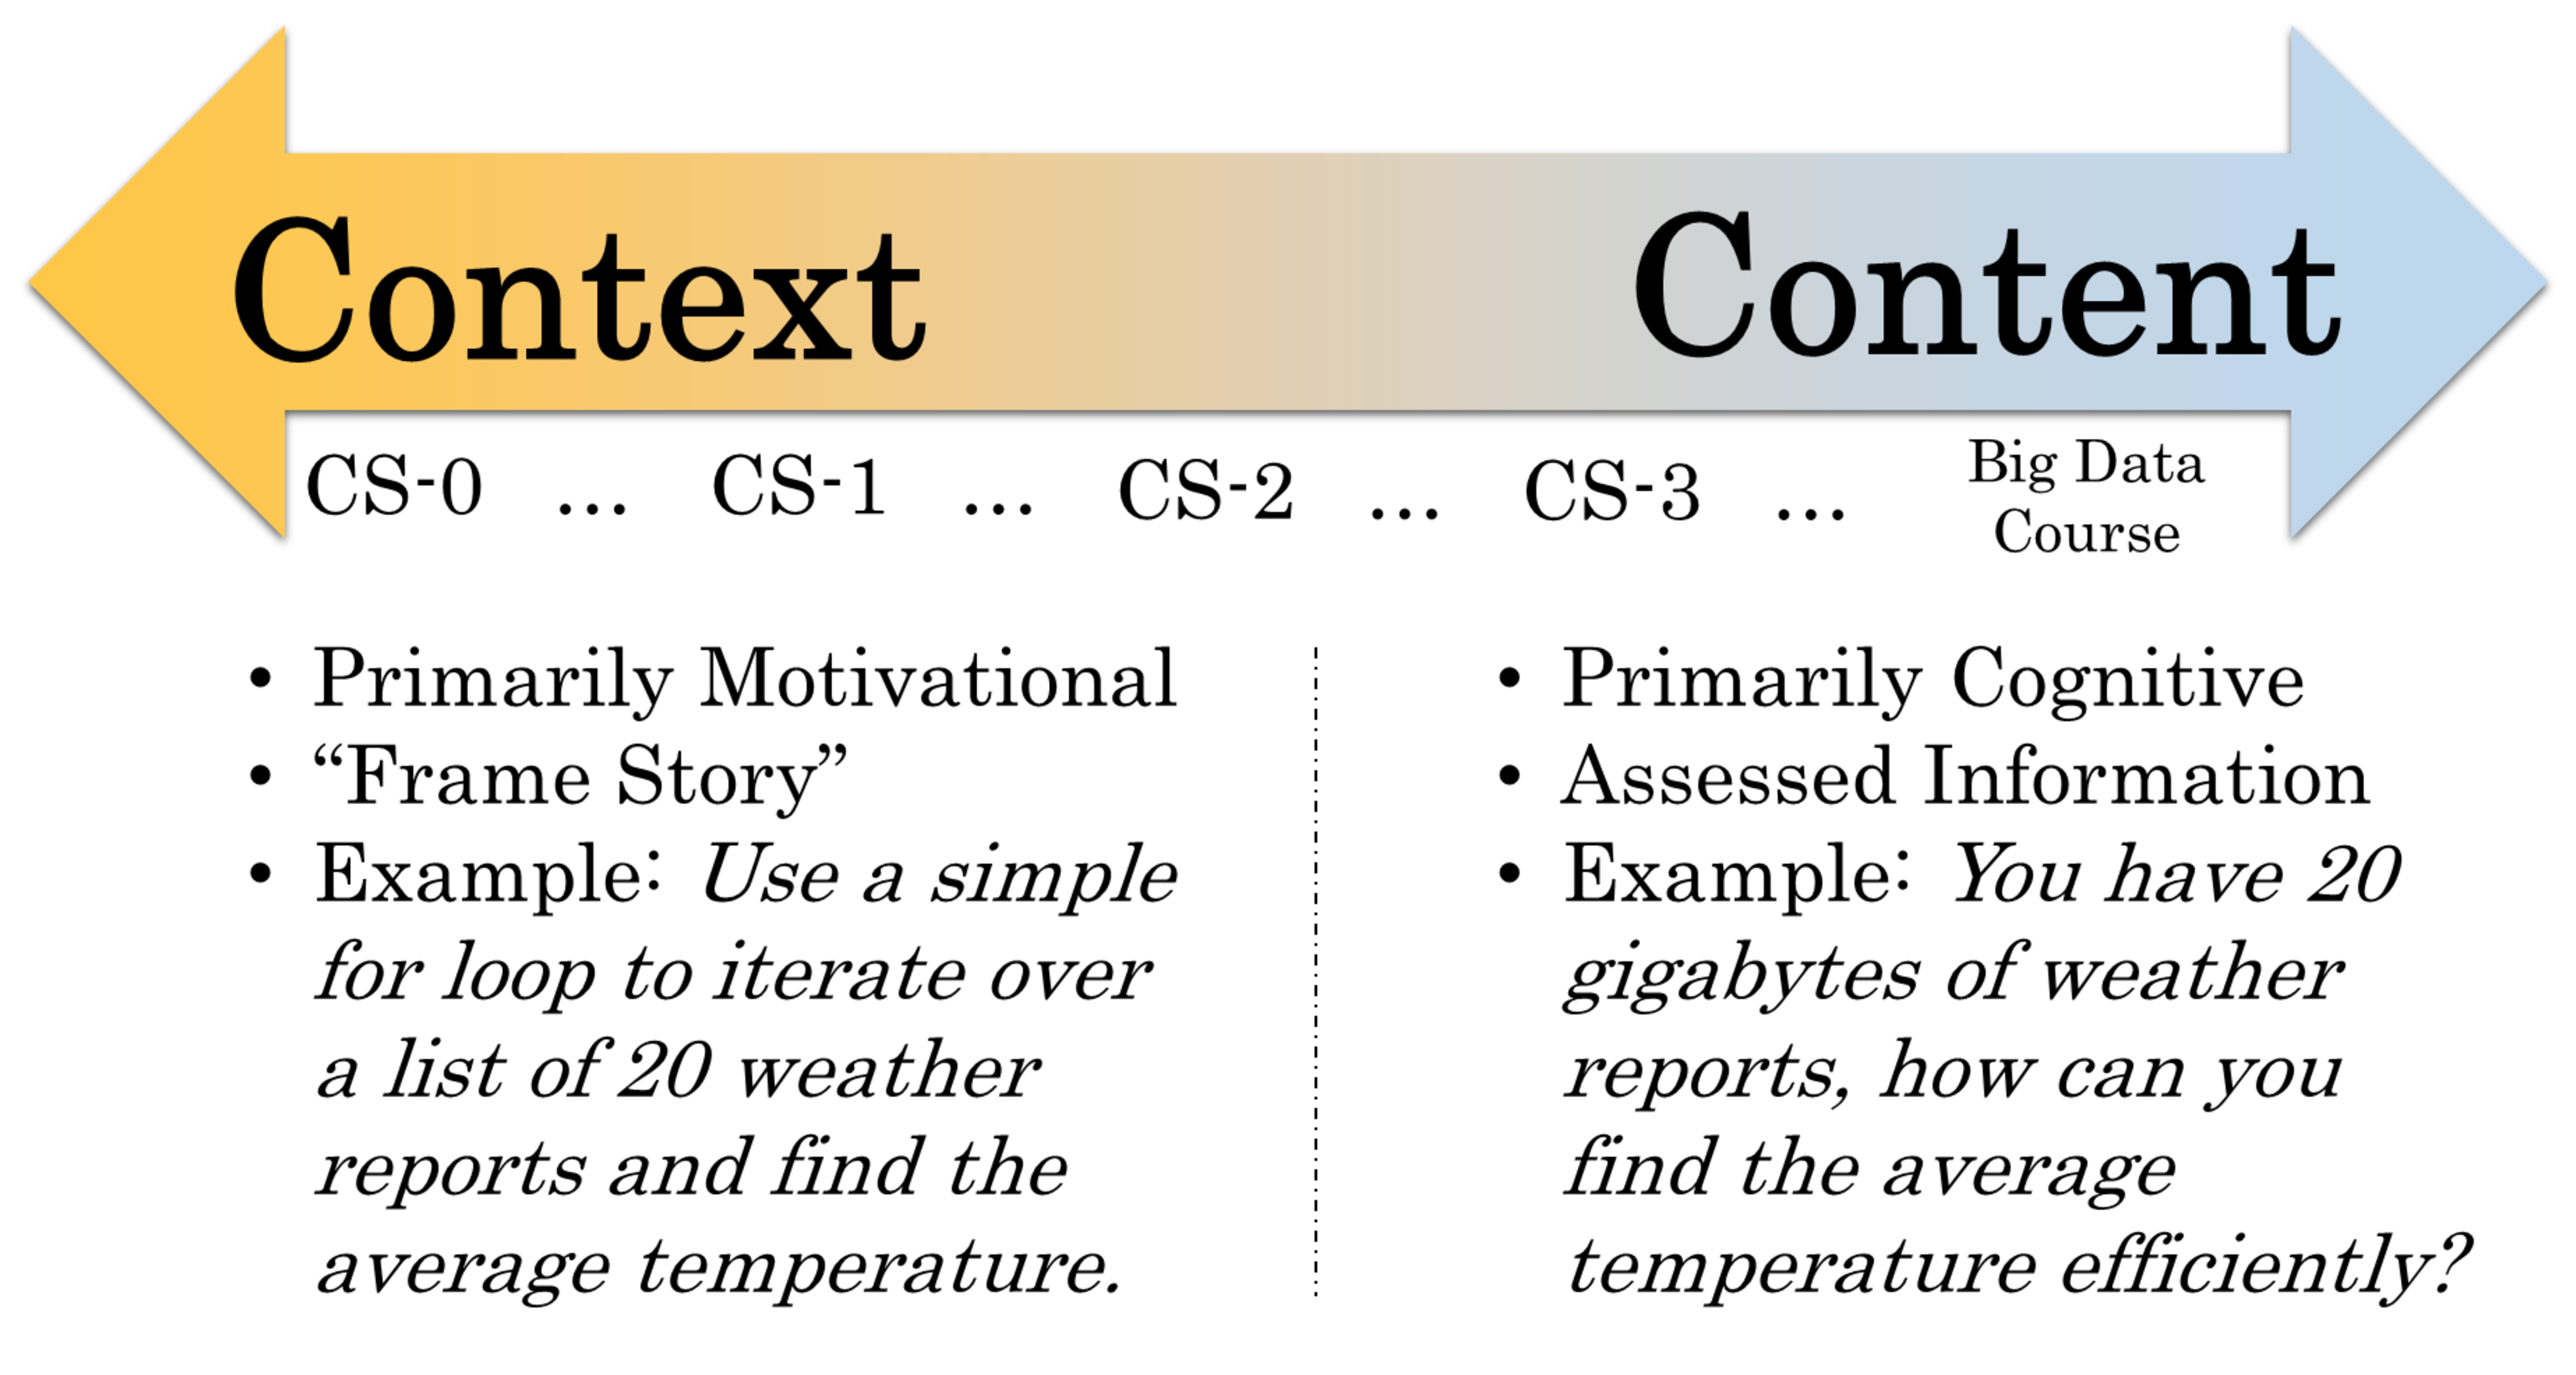
\psfig{file=images/content-context-2.eps, width=\linewidth}
		\end{center}
		\caption{Content vs. Context}
		\label{fig-content-context}
\end{wrapfigure}

\begin{description}
	\item[Context] ``... The problem's physical and conceptual structure as well as the purpose of activity and the social milieu in which it is embedded''\cite{rogoff1984everyday}, context is driven not just by the atmosphere of the problem at hand, but also by the background and culture surrounding the problem.
	A good context enables a student to find recognizable elements and build on prior understanding, eventually being able to freely transfer their learning to new contexts.
	\item[Content] The information intending to be conveyed to the students.
	If context is the backdrop to the learning, then content might be seen as the plot.
	Naturally, context and content are deeply intertwined with each other, and its difficult to talk about one without referencing the other; in fact, content is an abstract entity that needs to be made concrete through contextualization when it is delivered to the learner.
	If the information is too abstract, than it will never connect with the learner and will not be transferable to new domain.
	However, if it is too grounded in a domain, then it will not be clear how it can be re-applied elsewhere. 
	Ultimately, content must be given in a variety of forms to maximize transfer.
	Two useful methods for building content are anchored instruction (exploring scenarios, or anchors, in the context based on the content) and cognitive apprenticeship (mediating knowledge from an expert to the novice learner in a mentoring relationship).
	\item[Facilitations] The modifications to the learning experience that support and accelerate learning.
	Facilitations provide opportunities for students to internalize what they are learning by lowering the barriers that can surround situated experiences, possibly at the cost of some amount of authenticity. 
	These modifications might be technological in nature, but they can also be pedagogical.
	Although there are many different forms that Facilitations can take, Scaffolding is one of the most common.
	Scaffolding is a form of support that is intended to extend what a learner can accomplish on their own.
	This support is required at the onset of the learning process, but is unnecessary once a sufficient threshold has been passed; during this transition, the amount of scaffolding can be tuned to the learners understanding.
	In Computer Science, for instance, students often take advantage of software libraries and frameworks to create sophisticated graphical programs that would be beyond daunting if implemented from scratch.
	\item[Assessment] The methods used to assess the learning experience and the progress of the student.
	Choi \& Hannafin gives special attention to the “teach to the test” problem, and how assessment needs to change to measure students ability to solve authentic problem (as opposed to their ability to solve the test’s specific problem), and to be able to transfer their understanding when solving different but related problems.
	It is important that assessment is measured against the individualized goals and progress of a learner, requiring that any standards used be fluid and adaptable to different learners personal situations.
	Of course, assessment should be an on-going part of the learning process, providing feedback and diagnostics.
	Ultimately, the learner should join in the process of assessment as they transition to an expert – being able to meta-cognitively self-evaluate the effectiveness of ones methods and communicate results to others are key abilities of experts. 
\end{description}

There is a reciprocal relationship between contexts and content.
Figure \ref{fig-content-context} demonstrates an example of this relationship for the expected emphasis on big data as context vs. content throughout an undergraduate curriculum, from a CS-0 (non-majors) course all the way to an upper-level course specifically on big data.
Just as the upper-level course would naturally use big data as its context and content, a CS-0 course could still have content related to big data.
However, the majority of the use of big data would be as the framing story for assignments, especially in earlier parts of the course.
When students learn programming in the context of, say, game development, they are almost necessarily learning content related to game development that may not be universal to computer science -- e.g., how graphical resources are organized and accessed within the game engine.
This content may be seen as a distraction by the instructor, or as useful side knowledge - for example, if a student had to learn how to use a command line in order to compile their game, they would be learning an authentic skill that might not be considered part of the core content, but is nonetheless generally useful.
When evaluating a context, it is useful to consider what content it represents, and how authentic and useful it is.
The authenticity of content that is attached to a context affects the authenticity of the learning environment as a whole.

Fascinatingly, the need for a strong context diminishes as learners mature and become domain-identified -- the content itself becomes the context.
Learners start to see other contexts as nothing more than distractions and unnecessary fluff.
This makes sense -- you would hope that Computer Science majors in their third semester would be naturally interested in the material, and this is borne out in experimental data.
For instance, Yarosh \& Guzdial attempted to integrate Media Computation in a CS-2 (Data Structures) course, and found that the learners had ``outgrown the desire for a context''~\cite{yarosh2008narrating}. 
These results are similar to results we found in our interventions with a CS-3 (Data Structures and Algorithms), where students seemed more irked by the surrounding context than intrigued.

\begin{figure}
	\begin{center}
		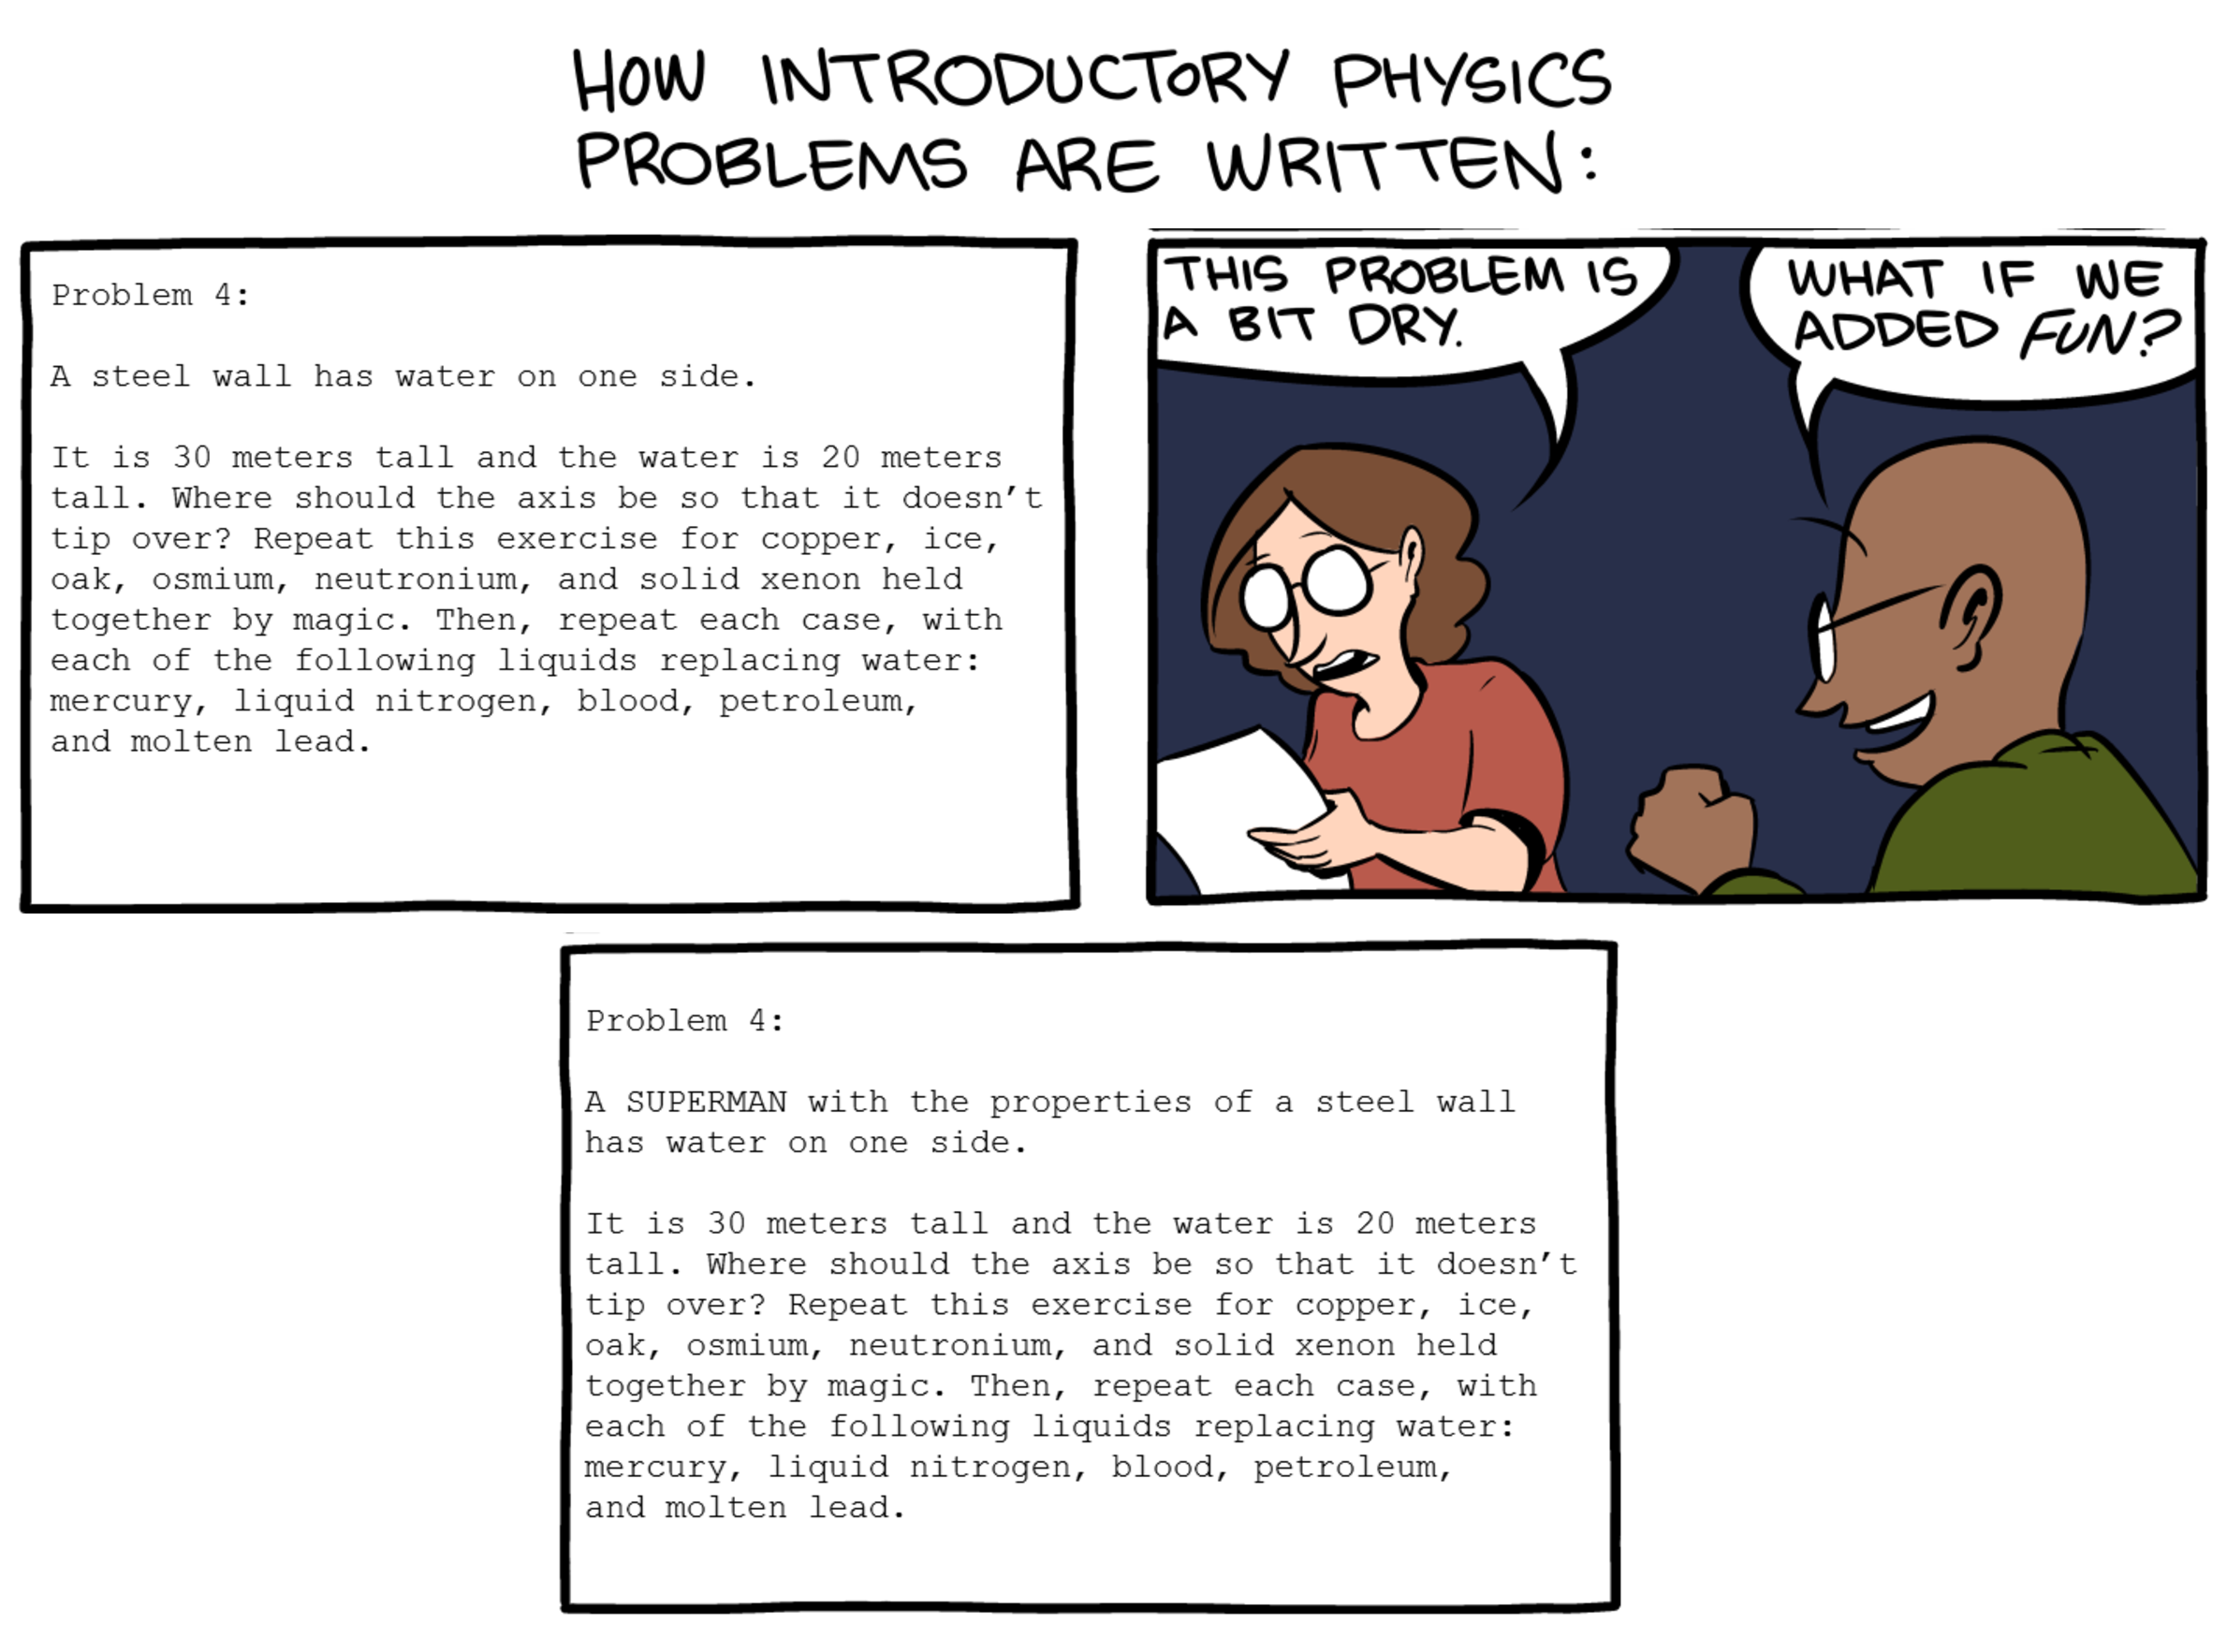
\psfig{file=images/smbc.eps, width=\linewidth}
	\end{center}
	\caption{Making the context ``Fun'' is not necessarily trivial, whether in physics education or computer science education.~\cite{SMBC}}
	\label{fig-comic-context}
\end{figure}

Of course, it is up to instructor to determine the depth and breadth of the context's integration.
The trade-off between the value and distraction added by the context is a delicate formula.
Consider the scenario in figure \ref{fig-comic-context}.
A steel wall is a relatively relatable concept for most students -- they can readily imagine such a large, durable object, and it somewhat reasonable to expect that objects would interfere with it.
In this scenario, the instructors consider replacing the wall with a comic book character -- something that they anticipate will be more ``fun''.
If they are in tune with their learners, this might actually be an effective context -- perhaps they know that their learners are comic book fans.
However, because the integration is only at the surface level, it is possible that the learners will see this as a forced reference, and they will have a more negative reaction.
It is also possible that they will not recognize the reference, or feel no positive emotions with it -- many contexts do not take into account gender, racial, or socio-economic characteristics of the anticipated learner.


\subsection{Theories of Motivation}

%TODO

\subsubsection{MUSIC Model of Academic Motivation}

Situated Learning is a theory of learning, but is not a comprehensive motivational framework -- it describes how people learn, but it is limited in explaining why people commit to learning.
Instead, it is useful to turn to the dedicated motivational models as a lens to explore why people choose to participate and excel in Computer Science.
In this preliminary proposal, we lean on the MUSIC Model of Academic Motivation as a primary framework.

The decision to use the MUSIC model was based on several criteria.
Although there are many motivational models available, few strive to be holistic models specifically developed for academics.
For example, theories like Expectancy-Value and Cognitive Evaluation Theory have a wider scope and have stemmed from other disciplines such as healthcare.
The MUSIC Model is derived from a meta-analysis of these other theories, incorporating only the academically relevant components.
Further, the MUSIC model is a tool meant for both design and evaluation, allowing it to be used in all phases of this work.
Finally, the model and its associated instrument, the MUSIC Model of Academic Motivation Inventory (MMAMI) , has been extensively validated and utilized in other educational domains, making it a reliable device\cite{jones-validity}.

The MUSIC model identifies five key constructs in motivating students \cite{jones-description}:
\begin{description}
	\item[eMpowerment:] The amount of control that a student feels that they have over their learning -- e.g., course assignments, lecture topics, etc..
	\item[Usefulness:] The expectation of the student that the material they are learning will be valuable to their short and long term goals. There is no clear delineation of the time-scale for these goals, but there is nonetheless a distinction between strategic skills that students need to be successful in careers and personal interests and the tactical skills they need to complete present-day tasks.
	\item[Success:] The student's belief in their own ability to complete assignments, projects, and other elements of a course with the investment of a reasonable, fulfilling amount of work.
	\item[Interest:] The student's perception of how the assignment appeals to situational or long-term interests. The former covers the aspects of a course related to attention, while the latter covers topics related to the fully-identified areas of focuses of the student.
	\item[Caring:] The students perception of other stakeholders' attitudes toward them. These stakeholders primarily include their instructor and classmates, but also can be extended to consider other members of their learning experience (e.g., administration, external experts, etc.).
\end{description}

Students are motivated when one or more of these constructs is sufficiently activated.
They are not all required to achieve maximal levels, and in fact that is not always desired -- it is possible, for instance, for a student to feel too empowered, and become overwhelmed by possibilities.
For some of these constructs, a careful balance is required, and it may not be possible to ever achieve a minimal level; no matter how exciting you make your lecture, you may never convince your students it is interesting, although it is possible that they will still consider it useful and stay motivated.
Much like in Situated Learning Theory, students' subjective \textit{perception} of these constructs is a defining requirement and is more important than objective reality.

The MUSIC model is often used as an organizational framework and an evaluative tool.
As the former, it is a list of factors to consider when building modules, assignments, and content of a course.
At all times, instructors can consider whether they are leveraging at least one construct to motivate their students.
As the latter, it offers both a quantified instrument (MMAMI) and a structure to anchor a qualitative investigation on.
The model has also directly been used tactically in course design: Jones describes a controlled classroom experiment to motivate students by having an experimental group reflect on how a course satisfies the constructs of the MUSIC model (e.g., prompted to answer ``How will the material presented here will be useful to you?'').
Quantitative data gathered after the experiment indicated a significant increase in motivation.~\cite{mcginley2014brief}

\subsubsection{Self-Efficacy}

Although the MUSIC Model is a holistic model, it can be useful to explore other theories of motivation that it draws on.
Self-efficacy is just such a theory, concerned with a learners judgment of their own capabilities.
Self-efficacy is often a strong predictor of students performance.
Students that believe they will fail will often do so, despite whatever ability they may have.

\subsubsection{Self-Regulation}
In the Self-Regulated Learning (SRL) model, learners succeed by actively practicing and developing their learning, willingly taking on challenging tasks, and reflecting on their strategies that lead to success.
In Computer Science, students must develop their understanding of how long programming tasks take, understand where their conceptual knowledge is weaker and believe that they can improve (as opposed to a fixed view), and a host of other meta-cognitive skills.
In an algorithms and data structures (CS3) course at Virginia Tech we have observed that students often have difficulty with the course programming projects.
These projects involve concepts such as dynamic memory allocation, recursion, file processing, differing interpretations of the bytes that represent data, and a collection of interacting classes.
The designs are more complex than students are used to, as the projects stress interacting classes requiring appropriate separation of concerns.
Too large a fraction of these students are unable to properly manage their time.
Research on procrastination [18, 19] indicates that motivation and self-efficacy for time management are key determinants for avoiding procrastination. In this project, we will provide big data as an available source of "inter-esting" projects.

\subsubsection{Extrinsic Motivation}

Although ideally, students will always be internally motivated to learn new subjects, this isn't always the case.
Academics are a careful balance of extrinsic and intrinsic motivation, with both internal and external rewards.
For instance, the ultimate goal of most formal education is certification, either by an accredited university or some other independent body.
In order to keep students on task, positive and negative grades are assigned based on performance.
Although these grades can drive negative behavior (e.g., nit-picking, arguments, etc.), they are ultimately necessary for some class of learners.
It can be a serious challenge for instructors to assign grades and use other forms of extrinsic motivation, to avoid dragging students along in a rigid environment but also not preventing students from floundering.
Too loose with a grading scheme, and students may deprioritize a course over stricter ones.
Too hard, and students may feel overwhelmed.
Although my research will not focus much on extrinsic motivation, it is important to understand its role in the classroom experience.
    \section{Introductory Computing Experiences}



\subsection{Content}

There is a serious, on-going debate about what novice students in computing should learn, with limited consensus. 
Complicating this discussion is the bifurcation of undergraduate introductory computing into Computational Thinking (sometimes referred to as CS-0) and Computer Science (sometimes referred to as CS-1), and the entirely different curriculum proposed for K-12 education.
There are some commonly agreed aspects however: any good introductory computing course will cover abstraction (representing complex phenomena more simply, usually as coded data), some form of decision-making (e.g., \texttt{if} statements, \texttt{cond} statements), and some form of iteration (e.g., \texttt{for} loops, recursion)~\cite{Kramer:2007, CS2013, csta-computational-thinking}.
From there, different curriculums lay out the material differently.
The ``How to Design Programs'' curriculum emphasizes a functional programming model, using a LISP-descended language named Racket, and the only looping mechanism that students are taught is recursion.
The dominance of the Object-Oriented Model in software engineering usually leads to a strong emphasis in introductory courses on abstracting data using Objects and Classes -- in fact, there is even an ``Objects First'' curriculum.
Of course, besides the technical aspects, definitions include softer skills such as a tolerance for unstructured problems and collaborative attitudes~\cite{csta-computational-thinking, google-computational-thinking}.

In general, this proposal will not take a strong view on what should be included in an introductory experience, beyond a core of Abstraction and Algorithms.
However, for practical purposes, materials and research work are grounded and tested in a course, and have adaptions for that content.
Specifically, this proposal is used in a Computational Thinking course, so that is how the content is oriented.
``Computational Thinking'' was coined by Seymour Papert in 1993~\cite{papert1996} and popularized by Dr. Jeannette Wing's 2006 paper~\cite{wing2006}, which opened a floodgate of discussion about the term. 
Unfortunately, there is still limited consensus on \textit{what} exactly CT is, whether it should be universally taught, how it should be taught, and how to identify when it has been taught.

An excellent resource for summarizing the history of Computational Thinking research is the 2013 dissertation by Wienberg~\cite{weinberg2013}. 
This comprehensive survey analyzed 6906 papers directly or indirectly related to Computational Thinking from 2006-2011, describing research efforts and findings.     
Over half of the research on CT describes approaches to pedagogy (Curriculum and Program Description), leaving a small amount to modeling (Philosophy and Opinion) and assessment (Research and Evaluation). 
The lack of assessment research is understandable given the youth of this area of research, but still troubling.
Even more troubling, however, is the further analysis of the 57 empirical studies.
Only fifteen (26\%) studies include or sought an operational definition of computational thinking, and only six go beyond the superficial (solely describing computational thinking as a "way of thinking", a "fundamental skill", or a "way of solving problems"). 
The failure to identify an operational definition weakens the theoretical strength of the studies.
This weakness likely stems from the background of the researchers: 28\% of the articles involved non-CS majors and \textbf{only 18\% of the articles involved education experts.} 
In other words, over four-fifths of this educationally-oriented research was performed by people with no real formal training in educational research techniques.
This is particularly troubling given that Computational Thinking is a strong target for interdisciplinary endevaors.

Weinberg reflects on the continuing debate about the importance of Computational Thinking:
\begin{quote}
    Many, like Wing, believe computational thinking to be a revolutionary concept, one as 
important to a solid educational foundation as are reading, writing, and arithmetic (Bundy, 2007\cite{bundy2007}) 
(Day, 2011\cite{day2011}). Others believe its potential and significance are overstated (Denning, 2009\cite{denning2009}; 
Hemmendinger, 2010\cite{hemmendinger2010}), and some have voiced concern that by joining forces with other 
disciplines computer science might be diluting either one or both of the participating disciplines 
(Cassel, 2011\cite{cassel2011}; Jacobs, 2009\cite{jacobs2009}). Both the praise and the criticism for computational thinking could 
perhaps be tempered by reflecting on a historical quote by Pfeiffer in 1962: “Computers are too 
important to overrate or underrate. There is no real point in sensationalizing or exaggerating 
activities which are striking enough without embellishment. There is no point in belittling 
either.” (Pfeiffer, 1962\cite{pfeiffer1962}).
\end{quote}

\subsection{Contexts}

As part of the overarching goal to bring more students into Computer Science, a large number of contexts have been explored in Introductory computing. 
The context of a learning experience grounds the learner in what they already known, in order to teach the new material.
Many introductory computing experiences focused on presenting the content as purely as possible, which can come across as abstract and detached~\cite{Zografski}.
However, starting with Seymour Papert's work with robotics and the LOGO programming environment in the 70s~\cite{papert1996}, instructors have been interested in motivating students' first experience with richer contexts.
Some of these contexts rely on Situational Interest (e.g.,  Digital Media ``Computation'' (Manipulation)~\cite{Forte} and Game Design~\cite{Zografski}), while others attempt to provide enduring career value (e.g., [Big] Data Science ~\cite{Anderson}) or short-term social applicability (e.g,. Problem Solving for Social Good~\cite{SocialGoodinComputingEducation}).
Ultimately, each of these approaches draws on different facets of motivation -- they do not partition the space, but reside in it organically depending on their implementation.
In this section, I will discuss the implications of these different approaches.


\subsubsection{Abstract Contexts}

Denning describes the early perception of Computer Science by the public as ``stodgy and nerdy''~\cite{Denning:2005}, since many early computer science classes were driven so strongly by mathematics and logic.
A common early introductory programming problem, for instance, is writing a function to compute a fibonacci number -- a relatively simple task if you are familiar with the recurrence, and one that leads quite nicely to discussions on the implementation of algorithms, computational complexity, and a host of other subjects~\cite{crazypantsfibonaccipaper}.
These contexts are ``abstract'' because they are already at a similar level of abstraction as the content they are attempting to convey.
However, Oliveira~\cite{ConcreteVsAbstract} suggests that the discussion about ``abstract vs. concrete'' contexts is a misleading one, because the purity with relation to the content is less important than \textit{prior knowledge}.
According to modern constructivist and cognitivist theories, learners build on prior knowledge, and the ability to relate to what they know is crucial.
The simple fact is that most students are not particularly good at mathematics, so relying on it as a context is not a useful approach compared to finding subjects that students know and understand readily.

\subsubsection{Situationally Interesting Contexts}

As it became clear that Computer Science had a serious image problem, work began on making Computer Science ``Fun'' and approachable. 
A key goal was to increase diversity and to broaden participation. 
This led to the rise of Situationally Interesting Contexts, emphasizing problems and projects that would be immediately appealing to a wide audience.
Guzdial, for instance, was largely responsible for the creation of the Media Computation approach, where students use computational techniques (e.g., iteration and decision) to manipulate sound, images, videos, and other digital artifacts.
As an example, students might use a nested, numerically-indexed \texttt{for} loop in order to adjust the red-value of the pixels in an image, treating it as a two-dimensional array of binary tuples, in order to reduce the red-eye of a photo.

Although wildly deployed, a review of these curricular materials by Guzdial \cite{guzdial2006imagineering} in light of Situated Learning Theory found that students did not find this an authentic context, and intense rhetoric was insufficient to convince them that it was authentic. 
Few students find it expedient and helpful to remove the red-eye from family photos by writing python scripts, when they could easily use a GUI-based program to automate the task instead.
Guzdial leaves open the question of what contexts can be truly authentic for non-majors, given the relative novelty of teaching introductory computing for non-majors.
Ben-Ari echos this question by suggesting a very narrow selection of authentic contexts and communities in his paper exploring the application of Situated Learning Theory to Computer Science in general \cite{ben2004situated}.
Critically, the opposite problem could occur -- if an instructor is effective at convincing students a context is authentic, they may believe them.
There are serious ethical issues involved in mispresenting the utility of a context, leading students to develop an embarrassing misconception of the field -- imagine a young child believing that all of Computer Science is game design, because that is what they started off doing.

There are other disadvantages of an Interest-driven approach.
The motivation literature describes ``Seductive Details'' (interesting but irrelevant adjuncts)~\cite{harp1998seductive} as interfering both with short-term problem completion and long-term transfer.
In other words, students get hung up on unimportant aspects of the context that they ignore the content.
Consider a student using the game and animation development environment Scratch, which allows beginners to create sprites from images.
A young learner may be so amused by the ability to change the color and shape of their image, that they neglect their assigned work.
Although a well-regulated learner would not be distracted, most of the at-risk population that would benefit from these contexts are unable to deal with such distractions.
Of course, this could be said of any context, but there is particular danger from this kind of context.

Kay~\cite{Kay:2011} identifies another, potentially critical problem of relying soley on situationally interesting contexts, particularly when it leads to individualized interest towards that context and not the content. 
What happens once a student has completed the introductory course and is ready to move onto further course?
Most later courses are more decontextualized, and will not use contexts such as game development, robots, etc.
Kay goes so far to say that it is unethical to suggest to students that a contextualized introductory course is representative of the curriculum as a whole.

\subsubsection{Empowered Contexts}

Orthogonal to the idea of making a context fun is the idea of giving students more freedom and agency to control their learning.
Compared to Interest-driven contexts, this approach is comparatively less researched, although it is not an uncommon practice -- instructors will often allow students to choose from a range of projects or assignments.
Stone~\cite{EmpowermentInProjects} ran a 2-year study where students were allowed to choose their projects from a wide range of domain areas (e.g., Biology, Math, Business, Etymology), and were then surveyed on their engagement.
Unfortunately, their experiment suffered strongly from low enrollments and even lower survey responses; it is difficult to believe any of their results (including the idea that women are more likely to prefer biological- and meterological-themed projects).
However, their experiences do suggest an interesting challenge: normalizing the difficulty (both in terms of computational knowledge and domain knowledge) across many different projects is a struggle.

\subsubsection{Useful-Driven Contexts}

An alternative focus to Interest is Usefulness, the idea that the context should have immediate or eventual benefit to the learner's needs.
To some extent, it is impossible (or at least prohibitively difficult) to find a one-size-fits-all context that will be useful to all learners (doing so is probably an example of preauthentication~\cite{preauthentication}, or designing learning experiences without your learners in mind).
The ideal situation for any instructor is to create contexts that specifically suit the interests and values of your learners~\cite{DiSalvo:2011}.
However, in practice, some contexts are broadly useful and are likely to engage a diverse crowd of learners.
In this section, I suggest two distinct contexts that might fall into this role: real-world problem solving and data science.

In theory, Computer Science provides tools for solving problems, and it is possible that the problem solving can be done with even the simplest tools~\cite{Layman:2007, Social-good}.
Many authors collaborated to produce a new framework centered around these ideas -- ``Social Computing for Good'', a collection of approaches and projects for interdisciplinary students to solve using computing ~\cite{Social-good}.
They raise a number of issues with using socially relevant materials: that games and graphics can be more appeal to instructors as a ``cheap'' source of motivation, that students and instructors can become cognitively overloaded by the addition of domain knowledge, and that instructors can even be intimidated if they don't have expertise in the domain area.
They also create a valuable rubric for developing and evaluating problems (which I map to elements of the MUSIC model below):
\begin{enumerate}
	\item The degree to which the problem is student-directed (eMpowerment)
	\item The amount of scaffolding needed (Success)
	\item The amount of external domain knowledge needed (Success)
	\item The contribution to the Social Good (Usefulness, Caring)
	\item The ``coolness'' or ``sexiness'' (Interest)
	\item The amount of explicit student reflection incorporated (Usefulness)
\end{enumerate}
Although this framework presents some ideas, there are still unsolved technical and pedagogical problems in how to optimally bring these materials to learners; their paper ends by raising questions about the effectiveness of this approach compared to existing methods.

A number of other researchers have created course materials, with varying degrees of evaluation.
Erkan~\cite{Erkan:2012} had a sustainability themed curriculum -- student surveys completed afterwards suggested some level of effectiveness, although the sample size (N=16) was far too small.
In addition to providing two case studies, Buckley ~\cite{Buckley:2008} suggests an interesting delineation between Social problems (uppercase S, indicating problems general to society) and social problems (lowercase S, indicating problems of personal interest to the learner).


Barker ran a large survey asking why students persist towards majoring in CS~\cite{Barker:2009} (N=113, only freshmen).
Critically, they found that Meaningful/Relevant Assignments (subsuming both Interest and Social Usefulness) was a major factor in whether students would persist in the major -- however, it wasn't one of the top ones.
Interestingly, whether students felt that their workload and pace was appropriate was a much bigger source of importance, suggesting that care and attention should be given to making a context suitably difficult before it is made interesting and useful.
This focus on ensuring normalized, appropriate difficulty is echoed by several other authors, all of whom suggest that doing so is not trivial~\cite{Rader:2011, Stevenson:2006}.

In the past two decades, the field of Data Science has emerged at the intersection of Computer Science, Statistics, Mathematics, and a number of other fields.
This field is concerned with answering real-world problems through data abstractions, and offer a less socially-conscious path to Usefulness.
As a context, there are pedagogical penalties for using it, since it introduces a wide variety of new content -- visualization, statistics, ethics, social impacts... the list is long~\cite{Anderson:2015-DP2}.
However, a good instructor can downplay the focus on these side-areas as needed, or even emphasize subject matter's strengths (e.g., a statistics major might find it interesting to use their mathematical background to strengthen their problem-solving investigation).
However, there are other difficulties: bringing in messy data requires real sophistication by the instructor, especially when working with Big Data.

The use of data analysis as a form of contextualization is not novel, and represents a new and actively growing movement where instructors create programming assignments with specific datasets in mind ~\cite{Anderson, Sullivan:2013, Hall-Holt:2015, DePasquale:2006}.
Upper division courses have employed these situated learning experiences using data of varying size and complexity for several years \cite{Egger, datamining, Waldman}.
However, in all of these research papers, there is typically very little evaluation of the advantages and disadvantages of using data science in introductory education.
Although Sullivan ~\cite{Sullivan:2013} did conduct a study on the difficulty and usefulness of the datasets they provided, they do not go very far in identifying lasting lessons for educators creating such datasets.
Other researchers conducted even less impressive studies: DePasquale~\cite{DePasquale:2006} included exactly ONE student response in their evaluation.

\subsubsection{Contexts that Make Instructors Care}

Most modern educational theories argue that learning is inescapably affected by social factors.
There is evidence that the instructor~\cite{thompson2009engine} and fellow students~\cite{Barker:2009} are the most important factors in an introductory experience, for instance.
Kay~\cite{Kay:2011} discusses this explicitly.
It is possible that the most important element in a context is not whether it is fun or useful, but whether the instructor can get excited about it and impart that enthusiasm to the student.
And not just enthusiasm, but a thorough understanding of the problem, its usefulness, and the rest of its attributes.

    \section{Big Data Science}

Big Data is much in the news these days, from reports of massive data
dredging by the NSA to tens of millions of credit cards stolen by
hackers from commercial databases.
Big Data has become crucial to scientific advances from understanding the
genome to predicting climate change.
Unfortunately, computer scientists in the workforce are woefully
unequipped for this shifting paradigm.
Indeed, a report by MGI and McKinsey's Business Technology Offices
declares that ``by 2018, the United States alone could face a
shortage of 140,000 to 190,000 people with deep analytical skills as
well as 1.5 million managers and analysts with the know-how to use the
analysis of Big Data to make effective decisions.''\cite{McKinsey}
There are many obstacles to effectively educating students on Big
Data.
Its representation, manipulation, and expression is
challenging, with modern curriculums and programming tools being
inadequate.

\begin{wrapfigure}{r}{0.5\textwidth}
    \begin{center}
		    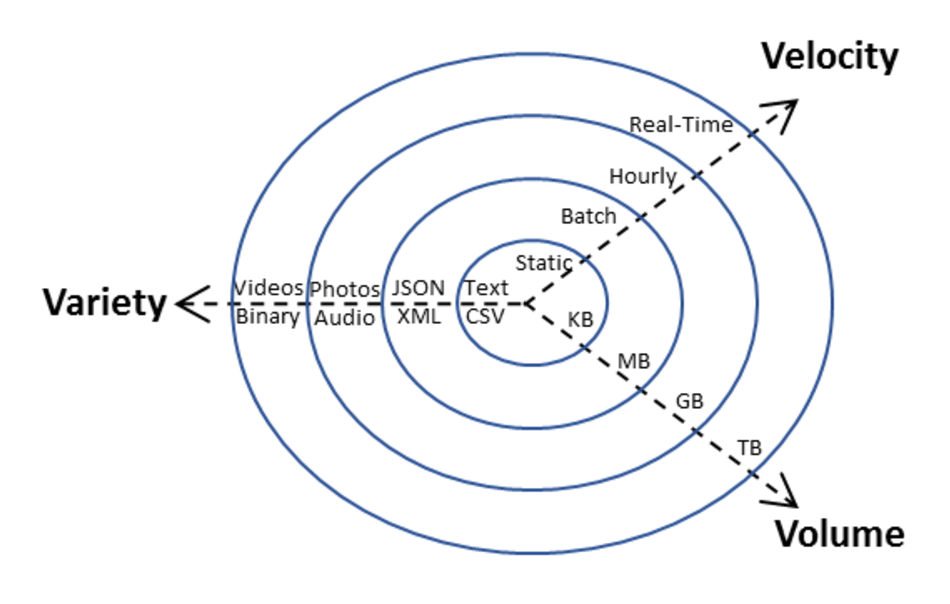
\psfig{file=images/3v-model.eps, width=\linewidth}
    \end{center}
    \vspace{-\bigskipamount}
    \caption{The 3V Model of Big Data}
    \label{fig-3v}
\end{wrapfigure}

Big data has been loosely described as quantities of information that cannot be handled with traditional methods ~\cite{McKinsey}.
But ``traditional methods'' is a vague phrase that has different meanings to different learners. To a Humanities major in their first CS-0 course, the traditional method to sum a list is to use Excel. In this scenario, ``big data'' means anything that won't comfortably fit into Excel's working memory.
However, to a third-year Computer Science major, the traditional method would be to write an iterative or recursive sequential loop; being given big data forces them to explore parallel models of execution.
Clearly, ``bigness'' is a function of the learner's experience, but that is still not a solid definition.

A more precise definition is the ``3V Model'' \cite{douglas2012importance}, which posits that there are three dimensions that distinguish big data from ordinary, run-of-the-mill data:

\begin{description}
	\item[Volume:] The total quantity of the information, usually measured in bytes or number of records. However, this also extends laterally: the number of fields in the structure of the data also impacts the complexity and size. The threshold at which data becomes big is a function of the hardware and software being used -- for instance, embedded systems may consider gigabyte-sized files to be big, while modern servers might not struggle until the petabyte level.
	\item[Velocity:] The rate at which new information is added to the system. High velocity big data implies a distributed architecture, since new data must be arriving from somewhere. The dynamicity of data can vary widely across these architectures, with data updating every year, every day, or even multiple times a second.
	\item[Variety:] The format or formats of the data. Ideally, data are always distributed in a way that is readily accessible -- for instance, simple text-based formats such as CSV and JSON are widely supported, relatively lightweight, and human-readable. More sophisticated data formats for image and audio are also typically well-supported, although still more complicated. However, projects using specialized, compressed binary formats or, more dangerously, multiple formats (e.g., image archives organized with XML files), are more complex.
\end{description}

In the remainder of this section, I describe common challenges associated with different kinds of data.

\subsection{High Velocity Data}

It is not trivial to enable introductory students to work with high velocity data, which is necessarily distributed. Without any scaffolding, it is necessary to delay the use of such data until much later in the course. In a prior paper \cite{realtimeweb-splashe}, we outline the biggest barriers to high velocity data as a context:
\begin{description}
  \item[Access] The process of programmatically downloading and parsing a web-based resource is a non-trivial procedure requiring an understanding of both basic concepts (e.g., function calls, data transformation) and specialized web technology (e.g., the difference between GET and POST calls, building query parameters).
	\item[Non-Idempotency] Because high velocity data is constantly changing, repeated calls to the same URL endpoint can return wildly different results, even over the course of a few minutes. This makes finding errors and testing considerably harder.
	\item[Consistency] Web-based APIs are controlled and developed by independent entities, which means that changes can occur at any time with little to no notification or time for reaction. This means that students' code can become out of date even during the middle of testing their final project.
	\item[Connectivity] Although internet speeds for students on a university campus are typically stable, this does not extend to off-campus students or students that are traveling. If the internet connection is down, then students might be completely unable to make progress.
	\item[Efficiency] Even when the internet connection is stable, it might not always be fast. Requiring a round-trip to a server can greatly drag on the testing and development process, frustrating the student and decreasing the time spent learning.
\end{description}

\subsection{High Volume Data}

In this section, we highlight some of the more challenging aspects of introducing high volume data, similar to how we previously outlined the challenges of high velocity data.
Some of these challenges are technical in nature, and some of them of a more pedagogical nature.
These challenges lead to certain design requirements that must be satisfied in any scaffolding intended to introduce high volume data.

\begin{description}
	\item[Data Transmission:] Internet connections can be difficult and inconsistent, especially for off-campus
and non-traditional students. Although most modern universities boast impressive wired connection
speeds, these speeds rarely extend off-campus. And even when internet connections are top-notch,
they can still be inadequate to serving the needs of transmitting big data collections to an entire
classroom of students. Some affordances must be made to make the data readily available to students without taxing their hard drives unnecessarily.
	\item[Different Contexts and Problems]: Additionally, high volume data offers different contexts and problems than high velocity data.
For instance, high velocity data typically lends itself to small quantities of data that are relevant to the current state of the real world -- for instance, students can walk outside and feel the current weather, which should correlate to real-time weather reports made available by a weather library.
High volume data, on the other hand, lends itself to large quantities of mostly static data -- for instance, crime reports for a long period of time.
Although high velocity data gives authentic answers in the here and now, high volume data gives authentic answers for the future, through trends.
Some fields have both kinds of data available -- meteorologists generate forecasts (high velocity, low volume) by studying historical climate data (high volume, low velocity).
But some fields are not amenable to both -- digital historians typically have large stores of historical information (high volume), but it does not change quickly (low velocity).
Careful consideration must be made when choosing problems and designing contexts so that the data leads to optimally authentic learning experiences.
\end{description}


\subsection{High Variety Data}

\begin{description}
\item[Inconsistency of Storage:] High variety data is composed of many different kinds of file formats -- some of which are more complicated than others.
\item[Inconsistency of Tools:] Different languages usually offer many different tools to interact with the exotic formats of the data -- however, these tools vary greatly in availability, usabililty, and compatability across platforms. For instance, binary image data is supported as a first-class programming object in the Racket programming environment, but can only be loaded using libraries such as Pygame in Python, which the user may or may not have installed.
\end{description}

\subsection{General Challenges of Data}

\begin{description}
	\item[Ensuring Wide Availability:] There is no universal agreement within the Computer Science Education community
on the perfect introductory language \cite{CS2013}. Indeed, individual instructor’s answers will change
depending on what CS course (e.g., CS-0 vs. CS-2) is being considered. Python and Racket/Scheme are growing in
popularity for CS-0/1, but Java is still a dominant choice for both CS-1 and CS-2 [8]. One of the great
successes of the RealTimeWeb project that we are building off was the availability of every API in at
least three common languages (Racket, Python, and Java). In order to ensure wide-spread adoption, our
new infrastructure must also be available in a number of commonly-used languages.
\item[Intentionally secured data] Organizations such as FERPA and HIPPA exist in order to ensure the privacy and dignity of captive populations (e.g., school children, patients). These organizations define rules for how data on such populations can be published and made available. Often, interesting data exists behind walled gardnes. Although novel techniques such as Differential Privacy (where data is probabilistically modified to protect anonymity) can be used to mitigate these problems, it is simply a fact that some data is utterly unaccessible.
\item[Unintentionally obfuscated data] Many developers have limited experience, time, and interest with the best way to package data for others' consumption. It can be easy to release a dataset as a PDF or in some obscure binary format. Overtime, data can also disappear behind dead/moved URLs. A major challenge for organizing data can be finding it and interpreting it.
\item[Non-uniform topologies] High volume data offers different contexts and problems than high velocity data.
For instance, high velocity data typically lends itself to small quantities of data that are relevant to the current state of the real world -- for instance, students can walk outside and feel the current weather, which should correlate to real-time weather reports made available by a weather library.
High volume data, on the other hand, lends itself to large quantities of mostly static data -- for instance, crime reports for a long period of time.
Although high velocity data gives authentic answers in the here and now, high volume data gives authentic answers for the future through trends.
Some fields have both kinds of data available -- meteorologists generate forecasts (high velocity, low volume) by studying historical climate data (high volume, low velocity).
But some fields are not amenable to both -- digital historians typically have large stores of historical information (high volume), but it does not change quickly (low velocity).
Similar differences exist with High Variety data -- understanding these trade-offs is cruical to using them effectively.
\end{description}

\subsection{Authenticity of Data}

Careful consideration must be made when choosing problems and designing contexts so that the data leads to optimally authentic learning experiences.
In practice, datasets can vary greatly in authenticity -- some data is collected incorrectly or has other errors, some data was predicted from a model rather than observed from real phenomenon.
A curious component of authenticity, however, is that it is a function of the observer.
A persuasive instructor might convince a class of students that an entirely artificial dataset was representative of real-world data, especially if it confirmed students' existing biases.
There are ethical issues with artificial datasets and the stories that they tell.
However, there are serious pedagogical benefits to generating datasets that fit instructor's goals -- data that leads to interesting visualizations, or clean results.
An important facet of my research will be exploring the ethical and pedagogical ramifications of the authenticity of datasets.

One of the big dangers when attempting to create meaningful context for learners is the problem of \textit{Preauthentication}: attempting to design for authenticity without sufficient knowledge of the audience. This is a problem shared by any approach to introductory material. Petraglia gives a compelling example \cite{preauthentication}:
	
\begin{quotation}
    The task of balancing a checkbook, for instance, may be an authentic task from the perspective of a 21-year-old, but we would question its authenticity from the perspective of a 5-year-old. But more to the point, even among 21-year-olds, for whom we believe the task should be authentic, there are some who will find any given lesson in personal finance irrelevant, inaccurate, or otherwise inappropriate. 
\end{quotation}
Preauthentication stems from over-generalizations and run-away assumptions.
If you attempt to reduce an entire classroom to a list of likes and dislikes, you run the risk of ignoring each individual learner's rich history and background that they will be building from. 
It is difficult to plan for and work against this ever-present danger when designing reusable assignments. 
Petraglia \cite{preauthentication} recommends that rather than attempting to design around students prior understanding, it is better to simply convince the learner of the authenticity of the problem.
But this is limiting, since it ignores the prior experiences and understanding that a student brings to their learning.
Instead, it would be better to find a middle ground where students are given flexibility while maintaining a relatively uniform experience for students.
In an ideal learning environment, students will have freedom to explore datasets of their own choosing, possibly from a list.
Of course, this must be balanced with the students inexperience with finding datasets, requiring the process be given time and attention.
    \section{Existing work}

As I am now three years into my PhD, my research builds on significant prior work. First and foremost, my CORGIS project has already been used in several introductory programming experiences, and seen publication at multiple venues, including two very successful workshops.
My primary research project for the first two years of my dissertation led to CORGIS: Collections of Real-time, Giant, Interesting, Situated Datasets.
This project's goal is to make simplistic data sources available to learners early in their programming experience, so that they can explore Big Data Science contexts.

\subsection{Technical Infrastructure}

\begin{wrapfigure}{R}{0.5\textwidth}
    \begin{center}
			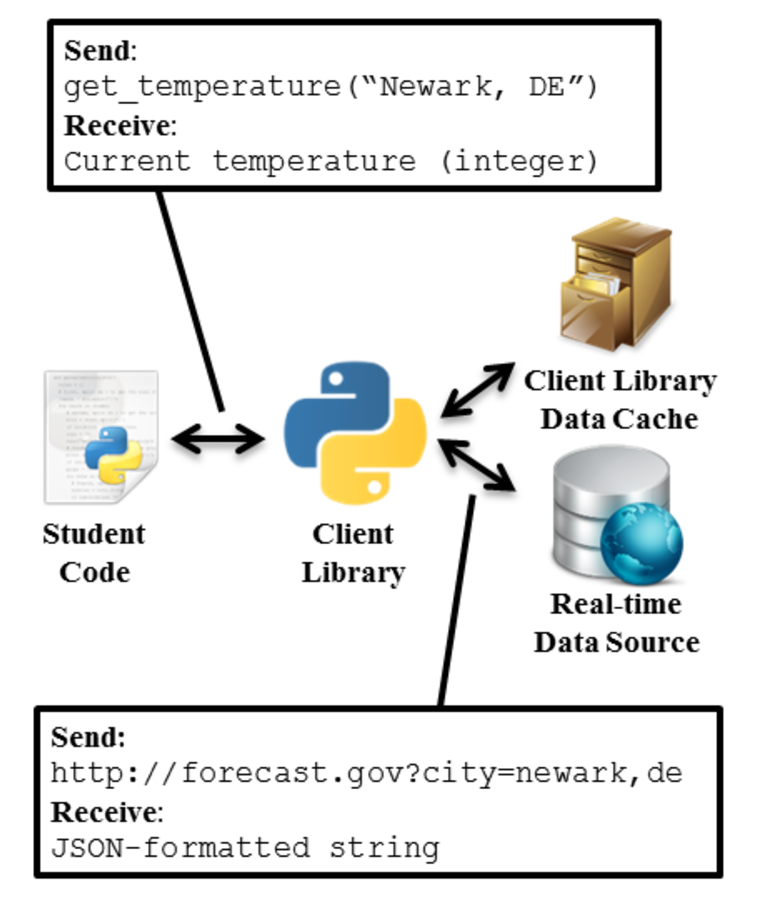
\psfig{file=images/rtw-client-library.eps, width=\linewidth}
			%\includegraphics[width=0.48\textwidth]{"images/rtw-client-library"}
    \end{center}
    \vspace{-\bigskipamount}
    \caption{RealTimeWeb Client Library Architecture}
    \label{fig-cla}
\end{wrapfigure}

The foundation of this proposal rests on prior work developing the RealTimeWeb project, a software architecture framework that provides introductory programming students with an easy way to access and manipulate distributed real-time data\cite{bart-transforming}.
Real-time data is a specific branch of Big Data -- specifically, high velocity data.

As our focus shifts from real-time data to datasets in general, we have renamed our overarching project from RealTimeWeb to CORGIS. Our work is now available at \url{http://think.cs.vt.edu/corgis/}. As a successor to the RealTimeWeb project, CORGIS retains all the previously developed libraries for accessing high velocity data; however, it also contains our new libraries for working with high volume data.
These libraries are paired with potential assignments and helpful documentation for deployment.
Long term, we intend to gather and disseminate data on the success of these libraries, with the hopes to establish a community of developers and educators that create new resources.
For clarity's sake, we use the name RealTimeWeb to refer to the architecture we have developed to rapidly connect to high velocity data streams.

At the heart of our project are carefully engineered, open-source client libraries through which students can access the data provided by real-time web services.
We provide client libraries for a number of data sources, such as business reviews from Yelp, weather forecasts from the National Weather Service, and social content from link-sharing site Reddit.com.
Each of these client libraries is in turn available for three common beginner languages: Java, Python, and Racket. 
These libraries do more than just streamline the process of accessing distributed data, however; each library is built with a persistence layer that enables the library to work without an internet connection.
Not only does this ensure that students without a solid internet connection can maintain productivity, it also simplifies developing unit tests. 
In fact, this technical scaffolding for the students circumvents most of the difficulties of distributed computing, including HTTP access, data validation, and result parsing.
Figure \ref{fig-cla} demonstrates the architecture used in our libraries.

The persistence layer is implemented using a caching mechanism, but not a traditional one.
In a conventional caching system, the result of every call made to the external service is memoized using a key-value store, often with a timestamp in order to expire out-of-date data.
In our caching system, an instructor preloads the cache with a sequence of data values for each expected call to the external service.
Although this limits the number of possible calls to the external service, it improves the consistency of the experience.
Instructors can specify policies for how the system returns data -- if the cache runs out, it could restart with the initial result, a developer-specified ``empty'' result, or repeatedly return the final result.
For example, consider the United States Geological Services' Earthquake data stream, which exposes a function to retrieve a list of earthquakes around the world for a given time period (e.g., past hour, past day, past week, etc.). 
The instructor could provide a cache to simulate a period of high seismic activity, returning a large number of earthquakes every time the function is called.
If the user exhausts the data in the cache, it might be programmed to return an empty list, signaling no further activity.

Our High Volume libraries often work by providing sampled versions of the data internally, so that students can work with faster, representative subsets.
Then, when they are ready for full deployment, they can switch to a ``full production'' mode -- trading speed for quality. 
Most of the work in developing these libraries is organizing the sampled data to load into memory and get processed as quickly and naturally as possible.

An alternative scheme for distributed High Volume libraries uses a more traditional caching strategy -- assuming that the data source is largely static, requests are cached locally.
This caching is typically done using a simple key-value store on the local filesystem.
Limits can be set on the size or lifespan of the data in the cache, allowing the system to update itself according to the velocity of the external data service.
Using open-source REST API generating tools such as Eve~\cite{Eve}, existing high volume datasets can be quickly transformed into distributed datasets, alleviating the issues of data storage and transmission.

\subsection{Semi-Automatic Library Generation}

Our client libraries are easily available through a curated, online gallery; each library is designed to be quickly adapted to instructors' specific academic desires. 
This gallery also provides a tool for rapidly prototyping new libraries based on our framework.
As an open-source project, we encourage collaborators to explore and extend the tools that we have created.

The process of connecting to online data sources is fairly uniform: performing an HTTP request to a URL returns formatted data (typically JSON or XML). 
This information must then be parsed into native data structures, and then filtered and transformed into an appropriate domain object using the language's proper construct (e.g., structs for Racket, classes for Java).
We've established a JSON-based client library specification file format that can be compiled to appropriate source code in each of the three target languages using the modern templating language Jinja2. 
This compiler can be easily extended to new languages by providing a template.
This specification format has two major components: the functions, which connect to the relevant URL endpoints, and the domain objects, that are generated from a successful HTTP request. 
This open-source tool has been used to successfully and rapidly develop a number of the existing client libraries.

\subsection{Contextualizing with CORGIS}

\begin{figure}
		\begin{center}
				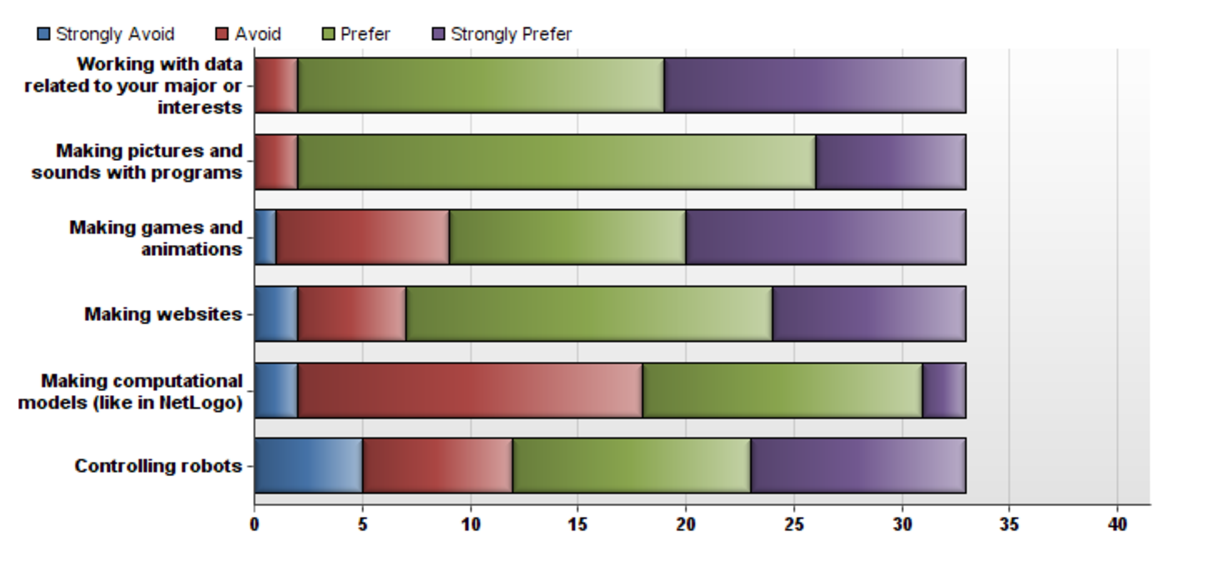
\psfig{file=images/contexts-compared.eps, width=\linewidth}
		\end{center}
		\caption{CT Students' Perceptions of the Appeal of Various Introductory Programming Contexts}
		\label{fig-contexts-compared}
\end{figure}

\begin{figure}
		\begin{center}
				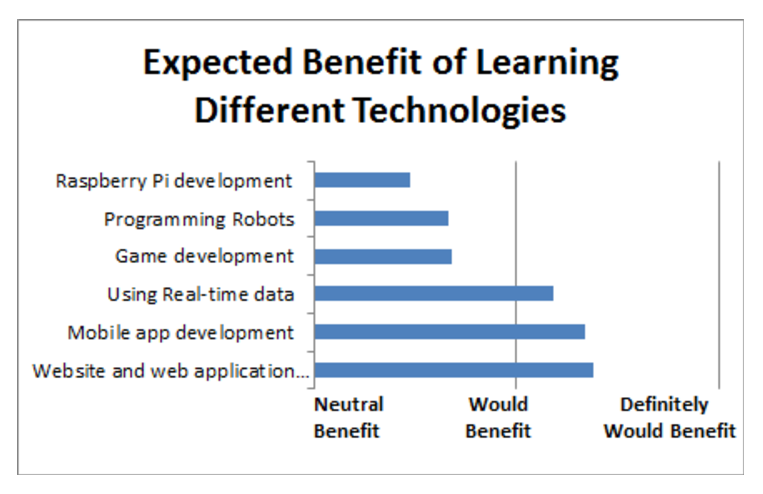
\psfig{file=images/expected-benefit.eps, width=.5\linewidth}
		\end{center}
		\caption{CS Majors' Perceptions of the Benefit of Working with Learning Different Technologies}
		\label{fig-expected-benefit}
\end{figure}

The CORGIS project has been deployed for several semesters in introductory Computer Science courses for majors, ranging from the first course all the way to a Data Structures level course.
These integrations ranged from small assignments to entire semester projects using the software.
So far, the focus of the evaluation has been on the motivational influence of the system.
Quantitative data was collected by surveying students attitudes using well-established motivational frameworks and instruments, and indicates that students tended to find real-time data engaging~\cite{realtimeweb}.
In some courses, qualitative data was gathered through small group interviews, where students attribute increased engagement with the authentic, real-world connection offered by real-time data.

Similar results have been found from its integration in a Computational Thinking course -- students cite working with the realistic data as a key factor in engaging with course materials.
Refer to figure \ref{fig-contexts-compared}, the result of an end-of-course survey (34 responses, 87\% response rate).
Students were asked to respond via a Likert scale to the statement, ``Other schools teach Computational Thinking in different ways. Consider these different styles, and indicate how much you would prefer or avoid them.''
Although this is an extremely shallow question, since students were only exposed to two contexts (computational modelling and working with data), it is an encouraging, preliminary result.

\subsection{Block-Based Programming}

\begin{wrapfigure}{R}{0.5\textwidth}
\label{fig-mlt-overview}
\psfig{file=images/graphics.ps, width=\linewidth}
\caption{The flow of code in the Mutual Language Translation system}
\end{wrapfigure}

Programming is a difficult thing to learn, and there exist many tools to scaffold that process.
One of the more popular approaches is Block-based Programming Environments, which allow the user to build their program from pieces of provided code constructs.
This prevents common syntax errors and some of the the ``blank canvas'' effect.
The CORGIS project has been leveraged in several different block-based environments, including a Python-based system based on Blockly and the popular programming environment/language Snap!. 
Both systems implement their own layer around CORGIS in order to provide access to rich datasets.
The Python/Blockly system has additional tools for creating plotted visualizations of data, and the Snap! interface has generalized support for accessing online data.
Although the Snap! tools were created as part of a spin-off project, the Python/Blockly tools are my own work.

During the Computational Thinking course, students take advantage of the internal caching mechanism of the CORGIS libraries to work on recorded data.
This simplifies the debugging process since programs perform predictably and are no longer dependent on external data services.
When students are ready to run their programs against live data, they can move offline to a traditional programming environment and run in regular production.
This caching mechanism also benefits from an assessment view - a students program can be checked for robustness by invisibly changing the values returned by the big data functions.
Figures \ref{fig-example-blockly} and \ref{fig-example-python} demonstrate the CORGIS library in action both in regular Python code and the equivalent Blockly code.

\begin{figure*}[hb]
\centering
\begin{minipage}[b]{.75\linewidth}
\caption{Blockly Code}
\label{fig-example-blockly}
\psfig{file=images/blockly-example.eps, width=\linewidth}
\end{minipage}

\smallskip

\begin{minipage}[b]{.75\linewidth}
\caption{Python Code}
\label{fig-example-python}
\begin{python}
import weather
import matplotlib.pyplot as plt

celsius_temperatures = []
for t in weather.get_temperatures("Miami, FL"):
	celsius = (t - 32) / 1.8
	celsius_temperatures.append(celsius)
plt.title("Celsius Temperatures in Miami")
plt.plot(celsius_temperatures)
plt.show()
\end{python}
\end{minipage}
\end{figure*}


\subsubsection{Authenticity of Data}

Careful consideration must be made when choosing problems and designing contexts so that the data leads to optimally authentic learning experiences.
In practice, datasets can vary greatly in authenticity -- some data is collected incorrectly or has other errors, some data was predicted from a model rather than observed from real phenomenon.
A curious component of authenticity, however, is that it is a function of the observer.
A persuasive instructor might convince a class of students that an entirely artificial dataset was representative of real-world data, especially if it confirmed students' existing biases.
There are ethical issues with artificial datasets and the stories that they tell.
However, there are serious pedagogical benefits to generating datasets that fit instructor's goals -- data that leads to interesting visualizations, or clean results.
An important facet of my research will be exploring the ethical and pedagogical ramifications of the authenticity of datasets.

One of the big dangers when attempting to create meaningful context for learners is the problem of \textit{Preauthentication}: attempting to design for authenticity without sufficient knowledge of the audience. This is a problem shared by any approach to introductory material. Petraglia gives a compelling example \cite{preauthentication}:
	
\begin{quotation}
    The task of balancing a checkbook, for instance, may be an authentic task from the perspective of a 21-year-old, but we would question its authenticity from the perspective of a 5-year-old. But more to the point, even among 21-year-olds, for whom we believe the task should be authentic, there are some who will find any given lesson in personal finance irrelevant, inaccurate, or otherwise inappropriate. 
\end{quotation}
Preauthentication stems from over-generalizations and run-away assumptions.
If you attempt to reduce an entire classroom to a list of likes and dislikes, you run the risk of ignoring each individual learner's rich history and background that they will be building from. 
It is difficult to plan for and work against this ever-present danger when designing reusable assignments. 
Petraglia \cite{preauthentication} recommends that rather than attempting to design around students prior understanding, it is better to simply convince the learner of the authenticity of the problem.
But this is limiting, since it ignores the prior experiences and understanding that a student brings to their learning.
Instead, it would be better to find a middle ground where students are given flexibility while maintaining a relatively uniform experience for students.
In an ideal learning environment, students will have freedom to explore datasets of their own choosing, possibly from a list.
Of course, this must be balanced with the students inexperience with finding datasets, requiring the process be given time and attention.

    \section{Proposed Technical Work}

To help support testing my hypotheses, a number of new pieces of technology and instruction will need to be created.

\subsection{Sophisticated Data Exploration}

Understanding the structure, meaning, and values of data can be a difficult problem for introductory students.
Using Data Science as the introductory context puts an increased emphasis on data structures and algorithms, making this content more critical for the learner.
Currently, there are not many tools available through Kennel to scaffold students.

The Property Explorer is probably the current greatest tool available to students for understanding program state.
However, field trials with it show that most students do not take advantage of the tool, with few reported events in the systems' tracker.
The usability of the property explorer, and its connection to the concept of Program State, must be elucidated to the student more clearly.

More tools are also desirable for engaging learners.
A number of graphical representations are used throughout the Computational Thinking course in order to visualize topics such as Abstraction and program flow.
For instance, students build Data Map Diagrams as seen in Figure \ref{data-maps-weather}, intended to help them navigate complex data structures.
The system can be extended to create simplified graphical visualizations of the students code and the data model in order to connect to these other course topics.

Currently, the implementation of MatPlotLib and other APIs is very minimal -- eventually, complete support for their functionality is needed.
There are other novel additions that can be introduced too -- for example, recent work by \cite{pixly} integrates media computation into Blockly environments.
By integrating such material into Kennel, we can provide students a comparative point between the different introductory programming contexts, in order to meaningfully evaluate the affordances of the different approaches.
Crucially, care must be taken to keep Kennel as a pure Python programming environment, without introducing cumbersome non-standard 3rd party libraries as occurs in CodeSkulptor~\cite{code-skulptor}.
As all of these materials extend the functionality of Kennel is new and innovating ways, but this material is less valuable if it reduces the authenticity and transferability of the learning experience.

\subsection{Complete Mutual Language Translation}

One of the biggest features of Kennel is the Mutual Language Translation, and this is where I expect a large amount of technical work will need to be done.
Indeed, there are a number of unsupported Python language features: classes are probably the biggest offender, but there are many other desirable features missing such as list unpacking, tuples, and sets.
These must be introduced to the system gradually and gracefully so that a beginner is neither overwhelmed nor distracted.
In some cases, incorporating these changes will require massive internal changes to Blockly's ability to represent concepts.

An ideal interface should offer a complete isomorphic mapping to Python - however, there are a number of complications to resolve before that can occur.
For instance, Python uses square brackets for both list indexing and dictionary access.
There is a strong desire to differentiate between these distinctive types of access, visible in the block view as two distinct kinds of blocks (``get ith element of list'' vs. ``get key from dict'' blocks).
Although some indexes are syntaxically unambiguous -- e.g., a string literal used as an index *cannot* be for a list -- there are many that are impossible to determine at compile-time using traditional static analysis.
This is largely because Python is a dynamic language -- the parser has no idea what type a variable has, so it is impossible to tell if a given variable is a dictionary or a list.
Instead, dynamic analysis needs to be combined with abstract interpretation techniques, such as those used in PySonar~\cite{PySonar}.
Typically these systems suffer from state explosion due to the large number of metaprogramming techniques usable in a python programmer - however, they are uniquely suitable for an educational environment due to the reduced subset of Python needed in practice by beginners.

A less technical and more user-oriented question is how many language details should be exposed, and what rate.
A rarely used feature of ``for'' loops in Python is to contain an ``else'' clause that is executed upon successful completion of the loop (that is, when it is not prematurely escaped using a ``break'' statement).
This advanced language feature is meant to draw special attention to connected actions that must be performed after the iteration is completed.
If an ``else'' clause were made available to beginners first trying to grapple with iteration, it is likely they would confuse the concept with the conditional ``else'' clause used in ``if'' statements.
Cognitive Load Theory can be a harsh mistress for beginners, and the user interface needs to avoid exposing unnecessary details where possible.
It can be very difficult to recognize when the learner is ready to understand parallel assignment, and therefore able to specify multiple variables on the left side of an assignment block.
This is actually an advantage of traditional text-based environments, since they hide all advanced features by their very nature.

However, there are techniques that can be applied to infer the types of most variables.
Simple dynamic analysis can be used to infer the type of a property over the course of the programs execution.
Certain restrictions can be made towards beginner's codes that, while draconian to an experienced developer, are reasonable for someone starting out.
For instance, we might require that a beginner only allow a property to take on a single type, issuing an error if they do not.
There are other edge cases that must be dealt with in a principled fashion.
It is impossible to predict the type output of ``eval'', for instance -- but fortunately, ``eval'' is bad practice in general and should also be forbidden to beginners.

\subsection{Meaningful Program Analysis}

In a classroom of many students and minimal instructors, it is a challenge to keep students successful.
Most students lack the programming knowledge to identify their own errors, let alone diagnose and fix them.
Although 1-1 human tutoring is ideal for learners, there are simply not enough staff resources.
For some kinds of problems, the system can support the student.

WebCAT\cite{webcat} is a well-known tool for solving this problem -- it uses style checks and unit testing to identify mistakes and make suggestions to the student.
There are other tests that can be used too.
A limitation of systems like WebCAT is that they often depend on a specific code shape: usually, they operate over explicit function contracts.
For example, students might be assigned to write a \texttt{sum} function which consumes an array of integers and returns a single value representing their summation -- students that do not match this contract can be guided.

Kennel already provides a limited API for providing such support, but it is extremely ad-hoc.
I propose a richer API for analyzing student code and tracking deficiencies.
Figure \ref{fig-example-analysis} provides a potential mock-up of this system.
The instructor implements a function that consumes some information about the students' code, and then returns feedback for the student and the system.
This API could additionally query for prior students mistakes, in order to provide more contextualized assistance -- if a student consistently iterated over an empty list, for instance, this could be representative of a greater understanding rather than a typo, and small hints would be less useful to their long-term learning than instructor intervention.

\begin{figure*}[ht]
\definecolor{mymauve}{rgb}{0.58,0,0.82}
\lstset{stringstyle=\color{mymauve}}
\lstset{
   language=JavaScript,
   backgroundcolor=\color{lightgray},
   extendedchars=true,
   basicstyle=\footnotesize\ttfamily,
   showstringspaces=false,
   showspaces=false,
   numbers=left,
   numberstyle=\footnotesize,
   numbersep=9pt,
   tabsize=2,
   breaklines=true,
   showtabs=false,
   captionpos=b
}
\begin{lstlisting}[columns=fullflexible]
function check(code, ast, variables) {
  // Did the student use too many or too few loops?
	if (ast.getIterations() != 1) {
	  // Give them a helpful message, and identify that they
		// made an iteration-related mistake.
	  return {'message': 'You are not iterating the right number of times!',
		        'mistakes': ['iteration']};
	}
	// Get the proper loop
	var iteration = ast.getIterations()[0];
	// Get the list we looped over
	var iteration_list= iteration.getList();
	// Check the state changes of the list over the program's life
	var list_states = variables[iteration_list];
	// Are they iterating over an empty list?
	if (isAlwaysEmptyList(list_states)) {
		return {'message': 'You are iterating over an empty list!',
		        'mistakes': ['iteration', 'program state']};
	}
	// Are they appending to the iterating list?
	if (changesAfterInitialization(list_states)) {
	  return {'message': 'You are changing at list as you iterate over it.',
						'mistakes': ['append']}
	}
	...
}
\end{lstlisting}
\caption{Analysis API Mock-up}
\label{fig-example-analysis}
\end{figure*}

In addition to the static program analysis, dynamic program analysis can also be used.
The custom libraries actually provide a useful mechanism for conducting behind-the-scenes unit testing.
A student submits code such as in \ref{fig-example-blockly}.
This code depends on a special CORGIS library that returns weather data, in particularly retrieving the weather for a specific city.
When the students code is evaluated by the system, this libraries functions can be repeatedly rerun to return different data -- substituting ``Blacksburg, VA'' as the argument, and ensuring that the students code returns the proper value.
This approach avoids more easily-abused output-checking, which students can fool by printing literal values as opposed to computed values.

Data Flow Testing can also be critically useful in evaluating students' code.
By observing the value changes that a property takes over time, common errors can be revealed.
The non-existence of an expected value can also be instrumentative.
A common beginner mistake is to not assign the output of an expression to a property -- either discarding the value entirely, or printing it instead.
A system could diagnose a missing value from the overall flow and suggest the user investigate the program state over time, or even revisit the lesson on the subject.

\subsection{Student Tracking and Reporting}

In order to scale the learning experience, instructors and course staff need to have access to a wealth of information about students.
No matter how involved and committed the staff is, they will be out-of-touch with some of these students.
This information involves motivation (do the students feel that they can succeed?), engagement (has the student been attending class?), ability (does the student understand iteration?), demographic (what major is this student?), and other dimensions of learning.
I propose creating a system, tied strongly to Kennel, to track students across as many dimensions as is useful and practical, in order to provide just-in-time reports for staff and the learners.

Much of this information needs to be made available quickly -- course staff cannot spare much time getting grounded on the history of the student.
During office hours, multiple students might show up at once.
A teaching assistant would wish to know who needs the most help, and what challenges individual students have already had.
For instance, a student might have already met with other TAs many times, indicating that they are struggling a lot in this course.
Although this is information that can be obvious with only a few minutes of interaction with the students, there is much time and energy wasted.

Course staff often meet regularly to assess the ``problem students'' and ``success students''.
The staff often make valuable estimations of their learners abilities and motivation, both in general and specifically.
This data could be captured by the system and used to drive the feedback being made available.
It can also be tremendously useful in course retrospectives.

The system can also assist in making interventions to support students.
Although hints and suggestions are obvious, there are other mechanisms too.
Students can be reminded of course goals that they have established (appealing to their long-term objectives).
Automated, self-regulatory suggestions can be sent to the learners when they have not engaged with the materials in a while, suggesting that they try out a problem for a while to see if they can make some progress (or at least identify their misconception) or move onto lateral material so they can make headway elsewhere.
Staff can be notified of a particularly struggling student, in order to encourage them to reach out with suggestions or encouragement.
Finally, situational interest could be appealed to with motivational content such as inspiring quotes, amusing images, or other rewards.

\subsection{More Libraries}

The CORGIS project depends on having an extensive and varied collection of datasets. 
Students should be able to find a dataset that appeals to their personal interests but provides a sound learning experience.
Making this experience relatively uniform is challenging, but makes providing support much easier -- a necessary element in a scaled classroom.

The same data source can be expressed in many ways, representing different levels of abstraction and different affordances.
Consider the data map in figure \ref{data-maps-weather}, representing potential structures for weather data collected about cities around the world.
Although maps A and B contain the exact same data, they are structured very differently -- a list of cities vs. a dictionary of cities.
For an experienced programmer, these differences are minor details that have implications for runtime performance: looking up a city's temperature is slower and more complicated in structure A (requring iteration and decision) than it is in B (requiring only dictionary access).
Although the differences in code are minor to an expert, they require fundamentally different areas of knowledge for a beginner.
Map C represents an entirely different level of abstraction, where weather is only represented as a numeric, without information about cities.
The number of questions that can be answered using this data is greatly reduced -- statistics about cities in general, rather than comparisons against specific cities.
And of course, the nature and schema of the data itself affects the types of questions that can be asked -- it makes sense to find the average of a list of temperatures, but not the sum.
A key part of my research will be explicitly identifies trade-offs and affordances of different structures and abstractions of data.

\begin{figure}
\begin{center}
\tikzset{
    bnode/.style = {   
        align=center, draw,
        rectangle split, rectangle split horizontal,
				rectangle split draw splits=false
    }
}
\begin{minipage}{.4\textwidth}
\begin{tikzpicture}
    \node[align=center, draw] (root)
		  {List of}
		;
		\node[bnode, below=of root,rectangle split parts=3]
       (middle)
       {	\nodepart{one}
					Dictionary of:
					\nodepart{two}
          ``city'' ,
					\nodepart{three}
					``temperature''
					};
		
    \draw (root) -- (middle);
    \draw (middle.two south) -- +(0, -1) node[draw, anchor=north](q) {string};
    \draw (middle.three south) -- +(0, -1) node[draw, anchor=north](q) {integer};
		%  +(0,-1) 
\end{tikzpicture}
\begin{center}
(A) List of Weathers
\end{center}
\end{minipage}
\begin{minipage}{.4\textwidth}
\tikzset{
    bnode/.style = {   
        align=center, draw,
        rectangle split, rectangle split horizontal,
				rectangle split draw splits=false, rectangle split parts=4
    }
}
\begin{tikzpicture}
		\node[bnode]
       (root)
       {	\nodepart{one}
					Dictionary of:
					\nodepart{two}
          ``blacksburg'' ,
					\nodepart{three}
					``newark'',
					\nodepart{four}
					``venice''
					};
		
    \draw (root.two south) -- +(0, -1) node[draw, anchor=north](q) {integer};
    \draw (root.three south) -- +(0, -1) node[draw, anchor=north](q) {integer};
		\draw (root.four south) -- +(0, -1) node[draw, anchor=north](q) {integer};
		%  +(0,-1) 
\end{tikzpicture}
\begin{center}
(B) Dictionary of Weathers
\end{center}
\end{minipage}


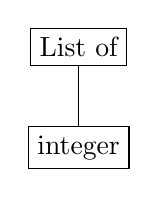
\begin{tikzpicture}
		\node[align=center, draw] (root)
		  {List of}
		;
		
    \draw (root) -- +(0, -1) node[draw, anchor=north](q) {integer};
		%  +(0,-1) 
\end{tikzpicture}
\begin{center}
(C) List of Temperatures
\end{center}

\end{center}
\caption{Weather Data Maps}
\label{data-maps-weather}
\end{figure}

Finding data sources can be a challenging task.
A component of my research plan is to publish best practices and techniques for finding, organizing, and exposing datasets.
The CORGIS collection already contains three dozen libraries, covering areas as diverse as international studies, nutrition, and social media platforms.
Some datasets were chosen because they were low-hanging fruit -- extensively documented, freely available, and well-supported. 
However, other datasets were driven by students' needs; in the two semesters that the course has been offered, two dozen new datasets have been created on demand.
The rapid turn-around time required has given new insight into the process of data mangling, although I am still exploring methods.
A massive part of my proposed work is to solidify and publish these techniques into a full paper.

    \section{Work Plan}

First semester
More data sources
Computational Thinking course data collection
Were students more engaged?
Self-report (MUSIC model)
Behavioral
more time on task
getting started earlier
further projects
integration into their own major work
Did students learn more? (UNSURE)
Improved assessments?
Not really sure this can be proven empirically from the data without some kind of standard measure.
Second semester
More data sources
Repeate measures for Computational Thinking
CS-1114 (CS-1)
Learning outcome changes
Behavioral
Increased retention
More time on task
Self-report (MUSIC Model)
Did they want more game dev? More media computation? Less RealTimeWeb?
Third semester
Further data collection

    \section{Work and Publication Plan}

This section outlines a schedule for my research over the next two years.

\begin{easylist}[itemize]
& Spring 2015
&& Second offering of CT course, collect baseline data (N=40)
&& Alpha version of Blockly/Python CORGIS integration
&& Second iteration of CORGIS libraries being used in a course
& Summer 2015
&& Preliminary Proposal
&& TOCE Journal Paper on Big Data Science Affordances
&& Beta version of Blockly/Python CORGIS integration
&& Block-based Language Workshop on Blockly/Python CORGIS integration
& Fall 2015
&& SIGCSE'16 Paper publicly announcing and describing Blockly/Python CORGIS integration
&& Third offering of CT course, collect data (N= expected 60-80)
& Spring 2016
&& Fourth offering of CT course, collect data (N= expected 80)
& Summer 2016
&& Development of second iteration of Blockly/Python CORGIS integration
&& Finalization of all major CORGIS architectures
&& TOCE Journal Paper on the design and issues of Virtual Learning Environments
& Fall 2016
&& Fifth offering of CT course, collect data (N= expected 80)
&& SIGCSE'17 Paper on affective/cognitive student tracking in Kennel
& Spring 2017
&& ITICSE'17 Paper, as a summative view of my primary research questions (using CORGIS to meaningfully motivate and guide large quantities of students to success).
&& Final Thesis Defense
\end{easylist}
    \section{Conclusion}

My research is focusing on motivating introductory computer science classes with broadly applicable contexts.
I seek to introduce new tools and approaches that can support instructors, developers, and learners in using data science and datsets as an introductory context.
In this preliminary proposal, I describe the technical work and how it will be deployed and evaluated in a Computational Thinking classroom.
I anticipate that this approach to introductory computing will provide useful new techniques and tools instructors.
The research results that I uncover will advance the literature in an crucial way.
    
    %\appendix
\newpage
\setcounter{page}{1}

    \bibliographystyle{abbrv}
    
    \bibliography{references}
        
\end{document}